\chapter{Diskussion der Umsetzung}
\label{chap:five}
Im folgendem Kapitel wird das Design des Prototypen besprochen und die Teilsysteme vorgestellt und skizziert wie die Teilsysteme
funktionieren. Dabei wird exemplarisch anhand von einzelnen Methoden der Klassen oder Funktionen beschrieben wie das funktioniert
Im Quellcode selber wird ausführlich jede Methode beschrieben.
\section{Implementierung}
    \subsection{Technische Details der Implementierung}
    Das Proof-of-Concepts wurde mittels der Programmiersprache Python umgesetzt.
    Python ist eine höhere Programmiersprache. Sie ist weitverbreitet \cite[vgl.][]{loukides_where_2021} und besitzt
    eine einfache Syntax. Besonderheiten von Python sind der Verzicht auf geschweifte Klammern und Interpunktionen nach Anweisungen.
    Die Anweisungen sind dagegen durch Einrückungen strukturiert und nicht durch öffnende und schließende Klammern
    getrennt. Des Weiteren zeichnet sich Python durch eine dynamische Typisierung aus und ist dadurch sowohl für Skripte als auch 
    für die schnelle Entwicklung von Anwendungen geeignet. Python erlaubt die Aufteilung von Programmen in Modulen, die in anderen Python-Programmen wiederverwendet werden können
    \cite[vgl.][]{python_6_2021}.
    Sie ist für alle wichtigen Plattformen frei verfügbar und verfügt über eine große Dokumentation \cite[vgl.][]{python_welcome_2021}.
    Wie andere Programmiersprachen besitz Python eine umfangreiche Standardbibliothek. 
    Dazu gibt es noch eine Vielzahl von Modulen, Programmen und Werkzeugen von Drittanbietern \cite[vgl.][]{python_pypi_2021}.
    
    
    Genutzt wurde für das Projekt insbesondere die Python-Bibliothek pandas, die eine Open-Source-Bibliothek für Datenanalyse und 
    Datenmanipulation darstellt \cite[vgl.][]{pandas_pandas_2021}. 
    Wichtige Konzepte dieser Bibliothek sind der pandas Dataframes und die pandas Series, die pandas Objekte sind. Der pandas Dataframe ist eine zweidimensionale 
    tabellarische Datenstruktur mit beschrifteten Achsen (Spalten und Reihen). In ihn
    werden die Daten unter anderem aus csv- oder xlsx-Dateien über pandas Funktionen geladen.
    Eine pandas Series kann Bestandteil eines Dataframes sein. Der Datentyp entspricht eines eindimensionales Arrays. \autoref{fig:pandas Dataframe und pandas Series} zeigt anhand der Umsatzdaten die ersten fünf Reihen
    eines pandas Dataframe und einer pandas Series desselben Dataframes. Zugriff auf die Series erfolgt über
    den Spaltenkopf 'Lieferant Abk.' der die Series über diesen anspricht. Sowohl der Dataframe als auch die Series haben einen Index, 
    über den auf die einzelnen Werte zugegriffen werden kann. 
    
    
    \begin{figure}[h]
        \centering
            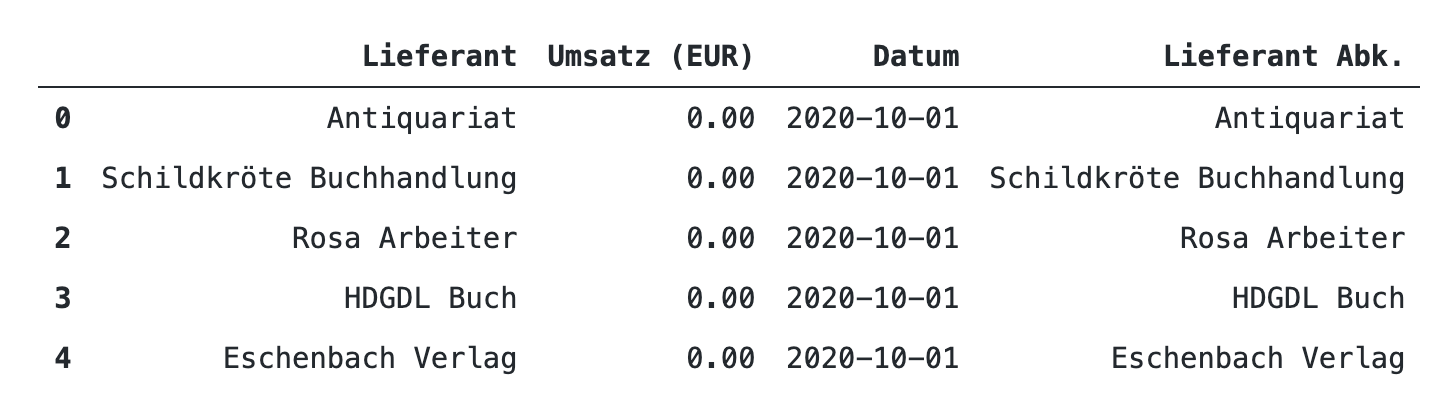
\includegraphics[width=7.5cm, height=3.0cm]{dataframe_example}
            \hspace{1cm}
            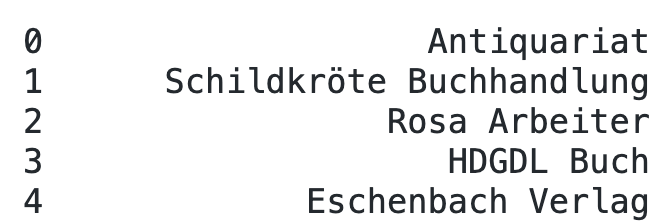
\includegraphics[width=5.0cm, height=3.0cm]{series_example}
            \caption{pandas Dataframe (links) und pandas Series (rechts)}
            \label{fig:pandas Dataframe und pandas Series}
    \end{figure}
    
    Auf dem Dataframe, der als sogenannter Container für die Series dient, können verschiedene Operationen der Datenanalyse und 
    -manipulation erfolgen. Ähnlich wie bei Abfragen einer Datenbank lassen sich verschiedene Funktionen wie \texttt{sort()}- oder \texttt{groupby()}
    in Zusammenhang mit Aggregatfunktionen wie \texttt{mean()}, \texttt{median()} oder \texttt{sum()} auf den Series durchführen.
    Auch gibt es eine Vielzahl von Funktionen, um Datasets rasch zu explorieren. Die Werte der Zellen können verschiedene Datentypen
    annehmen. Zum Beispiel können die Datumswerte der Spalte 'Datum' in \texttt{datetimeformat-Objekte} umgewandelt werden.

    In Verbindung mit pandas ist Python neben \textsf{R} und Matlab im wissenschaftlichen Kontext für Data-Science-Projekte sehr beliebt.
    
    Es gibt eine Vielzahl an Bibliotheken für Python, die für die Entwicklung von interaktiven Datenvisualisierungen verfügbar sind. Zu
    nennen wären Bokeh \cite[vgl.][]{van_de_ven_bokeh_2021}, Altair \cite[vgl.][]{altair_altair_2021} und die 
    Graphic Libraries von Plotly \cite[vgl.][]{plotly_plotly_2021}. Für das Projekt wurde sich für Plotly Express entschieden 
    und dieses hauptsächlich genutzt. 
    Plotly Express ist eine Graphische Bibliothek für Python, \textsf{R} und Javascript. Es ist eine Weiterentwicklung (Wrapper) der Bibliothek Plotly Graph Objects. 
    Plotly Express besitzt eine einfachere Syntax bei fast annäherender Feature-Gleichheit mit Plotly Graph Objects.\cite[][]{plotly_plotly_2021}.
    So können mit wenigen Zeilen Python-Code interaktive Grafiken erzeugt werden. 
    An interaktiven Basisfunktionalitäten bietet Plotly Express zum Beispiel Hover-Informationen der Datenpunkte, Zoom-In und Zoom-Out-Möglichkeiten,
    das Aus- und Abwählen von Balken oder Linien in den entsprechenden Diagrammen. Plotly Express kann pandas Dataframes 
    oder pandas Series als Datenobjekte erwarten und verarbeiten. Dabei können die Spaltenköpfe die Achsen darstellen 
    und die einzelnen Werte der Spalten die Datenpunkte bilden.Die Rendering-Engine für die Diagramme beruht auf dem JavaScript Framework D3.js. 
    Plotly Express ist frei verfügbar. In Kombination mit der Bibliothek Dash für die Entwicklung von interaktiven Dashboards lässt sich Plotly Express gut anwenden, 
    da beide von der selben Firma entwickelt werden und aufeinander abgestimmt sind. Mit der Bibliothek Dash wurde das Dashboard realisiert.
    
    Dash baut auf den Technologien Flask, Plotly.js und React.js auf. Das Framework ermöglicht die Erstellung interaktiver Webapplikationen 
    oder 'Analytical Applications' in Python ohne Javascript programmieren zu müssen \cite[vgl.][]{plotly_dash_2021}.
    Es gibt verschiedene Dash-Komponenten, die unterschiedliche Funktionen erfüllen. \texttt{Dash\_html\_components} stellen Klassen für alle HTML-Tags bereit.
    Die Schlüsselwortargumente dieser Komponente beschreiben HTML-Attribute wie style, className und id \cite[vgl.][]{plotly_dash_2021-2}. 
    Andere Komponenten sind \texttt{dash\_core\_components} oder \texttt{dash\_dependencies} \cite[vgl.][]{plotly_dash_2021-1}. Während die \texttt{dash\_core\_components}
    Steuerelemente und Graphen erzeugen, regeln die \texttt{dash\_dependencies} über Callback-Dekorator-Funktionen die Interaktion zwischen den einzelnen Komponenten.
    So kann zum Beispiel in der Dash-WebApplikation das Verhalten eines Diagramms von den Werten eines Dropdown-Menu gesteuert werden. 
    % Die zugehörige Callback-Dekorator-Funktion wird in diesem Falle automatisch von Dash aufgerufen, sobald sich der Wert des Dropdown-Menüs ändert. 
    Dabei bewältigt Dash alle Javascript-Anforderungen im Front- und im Backend \cite[vgl.][]{plotly_dash_2021-3}.
    \texttt{Dash\_bootstrap\_components} ist eine weitere Bibliothek, die zum Einsatz in diesem Projekt kommt. Sie unterstützt die grafische Umsetzung
    des Dashboardes \cite[vgl.][]{faculty_dash_2021}.

    \autoref{tab:Software-Requirements} zeigt einen kurzen Überblick über die Versionsnummern der genutzten Programmiersprache und der hauptsächlich 
    genutzten Bibliotheken sowie deren Open-Source Lizenzen.
    
    \begingroup
        \setlength{\tabcolsep}{4pt} % Default value: 6pt
        \renewcommand{\arraystretch}{1.5}
        %\resizebox{\textwidth}{!}{
        \begin{table}[h]
            \centering
            \begin{adjustbox}{max width=\textwidth}
            \Huge
            \begin{tabular}{lccl}
              %\begin{tabular}{p{3cm}p{5cm}p{1cm}p{1.5cm}p{2cm}p{4cm}}
               \toprule
               \textbf{Name}             &{Version}    &\textbf{Lizenz}                        & \textbf{Webseite}\\
               \midrule     
                    Python               &3.7.9         &Open Source (PSF)                     & \url{https://docs.python.org/3.7/}\\
                    pandas               &1.1.5         &3-Clause-BSD-License                  & \url{https://pandas.pydata.org/pandas-docs/version/1.1.5/}\\
                    Plotly               &4.14.1       &MIT-License                           & \url{https://plotly.com/python/}\\
                    Dash                 &1.18.1        &MIT-License                           & \url{https://dash.plotly.com/}\\


                \bottomrule
            \end{tabular}
            \end{adjustbox}
            \caption
            \label{tab:Software-Requirements}
            }
             \end{table}
        \endgroup
    
     
    \subsection{Systemarchitektur}
    
    Das System teilt sich in drei Teilsysteme auf, die im \autoref{chap:five_one_three} näher beschrieben werden. 
    \autoref{tab:Teilsysteme} zeigt die drei Teilsysteme mit einer Kurzbeschreibung der Hauptaufgabe.
    Teilsystem 1 ist für die erste Bereinigung der Daten und den Import der Daten in ein einheitliches Datenformat verantwortlich. 
    Teilsystem 2 greift auf den Speicherort der importierten Dateien zu und bereitet die Daten für die Anzeige im Dashboard vor, 
    indem es mit der Python-Bibliothek pandas Daten vorfiltert, gruppiert und Berechnungen auf den Daten ausführt. Teilsystem 3 ist für das Layout des Dashboards, 
    die Erstellung der Diagramme, die Anordnung der Diagramme im Dashboard, die Bereitstellung von Interaktionen mit dem Dashboard im Frontend
    verantwortlich. Teilsystem 1 und Teilsystem 2 wurden versucht objektorientiert zu programmieren, da hier der Anspruch bestand, den Programmcode
    für verschiedene Daten wiederzuverwenden. Teilsystem 3 besteht vorerst nur aus Funktionen, die die Anzeige im Frontend ermöglichen.
    %Teilsystem 4 besteht dahingegen wieder aus objekt-orientierter Programmierung. Genutzt wird hier eine Library, die OOP vorgibt. 

       \begingroup
            \setlength{\tabcolsep}{4pt} % Default value: 6pt
            \renewcommand{\arraystretch}{1.5}
            %\resizebox{\textwidth}{!}{
            \begin{table}[h]
                \centering
                \begin{adjustbox}{max width=\textwidth}
                \Huge
                \begin{tabular}{cll}
                  %\begin{tabular}{p{3cm}p{5cm}p{1cm}p{1.5cm}p{2cm}p{4cm}}
                   \toprule
                   \textbf{Teilsystem}             & Name   &{Hauptaufgabe} \\
                   \midrule     
                            1                      &Import  &Import und erste Bereinigung der Daten aus heterogenen Datenquellen.\\
                            2                      &Datenbearbeitung     &Aufbereitung der Daten für die graphische Darstellung im Dashboard.\\
                            3                      &Darstellung          &Umwandlung der Daten in Datenvisualisierungen und Implementierung der Dashboard-Logik.\\
                        %   4                      &Standardbericht      &Export ausgewählter Datenvisualisierungen und Darstellung in Berichtsform.\\

                    \bottomrule
                \end{tabular}
                \end{adjustbox}
                \caption
                \label{tab:Teilsysteme}
                }
                 \end{table}
            \endgroup
    

    \subsection{Teilsysteme}
    \label{chap:five_one_three}
    \textit{Teilsystem 1 Import}\\
    Das Teilsystem Import ist verantwortlich für den Import der Daten im Rohformat aus vordefinierten Importverzeichnissen 
    in vordefinierte Zielverzeichnisse. Das Ziel ist einerseits die Daten automatisch ohne Informationsverlust zu importieren 
    und andererseits diese mit notwendigen Daten für die weitere Analyse anzureichern und erste Bereinigungen der Daten durchzuführen. 
    Die Daten werden zum Abschluss im csv-Format abgespeichert. Mit dem Teilsystem soll eine einheitliche Datengrundlage für die spätere 
    Bearbeitung und Darstellung der Daten garantiert werden. Für das csv-Format wurde sich aufgrund seiner flachen und einfachen Struktur, der guten Lesbarkeit
    und seiner weiten Verbreitung entschieden.
    % Die Daten werden jeweils in ein pandas Dataframe geladen. Das Dataframe wird dann verschiedentlich bearbeitet, bevor es zum Schluss als csv-Datei in dem jeweiligen
    % Zielverzeichnis abgespeichert wird.
    Das Teilsystem Import besteht aus vier Klassen. Die \autoref{fig:classes import} zeigt die einzelnen Klassen mit ihren Methoden.
    Die Klassen im Teilsystem Import sind auf die Daten aus fremden Quellen zugeschnitten
    (Budget Umsatz, Neuerwerbungslisten, Ausleihe (Anwendungsfall 2, 4-6)). Dennoch können mit mit ihnen auch die bibliotheksinternen Daten
    wie Lesesaalnutzung (Anwendungsfall 3) bearbeitet werden. 
    \begin{figure}[H]
        \centering
            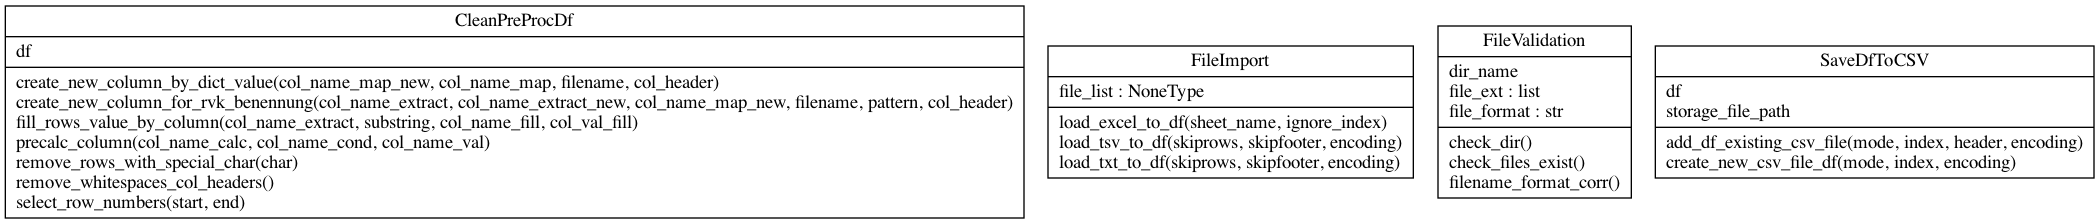
\includegraphics[width=14cm, height=3.5cm]{classes_imp}
            \caption{Klassendiagramm - Teilsystem Import}
            \label{fig:classes import}
    \end{figure}

    Instantiiert werden die einzelnen Klassen für die jeweiligen konkreten bibliothekarischen Daten in eigenen Python Skripten. 
    So gibt es Skripte für Budget, Umsatz, Ausleihe und Bestand/Neuerwerbungen. Diese verwenden für die Daten passende Methoden
    und führen den Import durch.
    Den Ablauf des Teilsystems zeigt schematisch die \autoref{fig:flow import}.

    \begin{figure}[H]
        \centering
            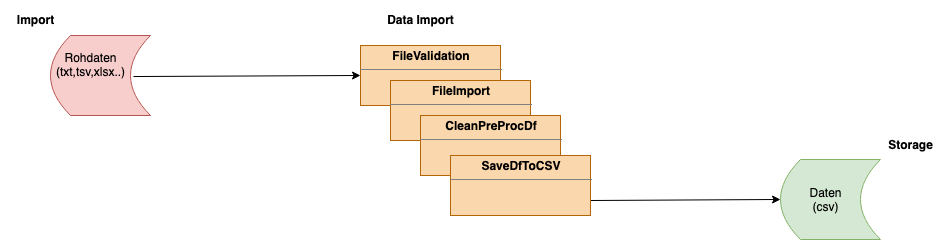
\includegraphics[width=12cm, height=3.5cm]{flow_imp}
            \caption{Datenfluss - Teilsystem Import}
            \label{fig:flow import}
    \end{figure}

    
    (1) Für den ersten Schritt sind die Klassen \texttt{FileValidation} und \texttt{FileImport} verantwortlich.
    Die Dateien werden aus einem lokalen Verzeichnis in ein pandas Dataframe geladen. 
    Dabei wird mit den Methoden der Klasse \texttt{FileValidation} überprüft, dass sowohl das Verzeichnis als auch die Dateien existieren. 
    Des Weiteren wird sichergestellt, dass die Dateinamen einem definierten semantischen Format wie dem Datumsformat YYYY\_MM\_DD und 
    einem Dateiformat wie txt-, xlsx- oder tsv-Format entsprechen. Wenn die Daten nicht diesen Vorgaben entsprechen, werden sie nicht in
    das pandas Dataframe geladen. Da die Daten unterschiedlich aufgebaut und in unterschiedlichen Dateiformaten vorliegen 
    werden beim Laden in den Dataframe jeweils verschiedene Methoden angewandt, dabei werden spezifische pandas-Funktionen eingesetzt,
    die die diese Datenformate bearbeiten können. 
    
    Beim Ladeprozess der Dateien in den pandas Dataframe wird mit den Methoden \texttt{load\_txt\_to\_df()} oder \texttt{load\_tsv\_to\_df()} 
    der Klasse \texttt{FileImport} der Dateiname von der Datei extrahiert und in einer neu geschaffenen Spalte des Dataframes im Datumsformat YYYY-MM-DD gespeichert.
    Anhand den Werten dieser Spalte werden später verschiedene Datenanalysen und Datenvisualisierungen vollzogen.\footnote{Dieses Verfahren wird bei den Daten ausgeführt, die einer zusätzlichen Datumsspalte bedürfen.} 
    Verantwortlich für die Extrahierung des Dateinamens ist die in \texttt{utils.py} ausgelagerte Funktion \texttt{date\_from\_filename},
    die den Dateinamen als Argument entgegennimmt.\footnote{In der Datei \texttt{utils.py} sind noch andere Funktionen als stand-alone-functions für den Datenimport und Datenbearbeitung gruppiert,
    da diese das Objekt \texttt{self} nicht verändern.} 
    
    (2) Das geladene pandas Dataframe wird im zweiten Schritt durch die Klasse \texttt{CleanPreProcDf} aufgenommen und durch verschiedene Methoden dieser Klasse
    manipuliert. Beispielhaft ist hier die Methode \texttt{create\_new\_column\_for\_rvk\_benennung} zu nennen, die aus der Spalte der Signatur 
    der Neuerwerbungen die Hauptklassen der \textit{\acrlong{RVK}} extrahiert und in einer neuen Spalte speichert. Dieser Methode liegt eine csv-Datei
    der \textit{\acrshort{RVK}} zu Grunde, die mit einem Skript aus der \textit{\acrshort{RVK}}-XML-Datei entstanden ist. Manuell ergänzt wurde diese 
    noch um selbstgeschaffene Hauptklassen der Institutsbibliothek. Die Methode wird sowohl bei den Neuerwerbungs- und Ausleihdaten angewendet.
    Ebenso entstehen neue Spalten bei Umsatz- und Budgetdaten. In Bezug auf die Darstellung der Daten im Dashboard werden
    hier die Namen der Lieferanten und Kostenstellen in lesbarer Form in einer neuen Spalte gespeichert. 
    Des Weiteren gibt es in der Klasse \texttt{CleanPreProcDf} Methoden, die für die Entfernung von Reihen mit bestimmten syntaktischen Zeichen wie Bindestrichen 
    verantwortlich sind oder die eine Vielzahl unnötiger Leerzeichen in Spaltenköpfen löschen durch ein Leerzeichen ersetzt.
    Ferner werden erste Berechnungen auf den Daten ausgeführt, um valide Daten für die Auswertung zu haben. Dies betrifft die Ausleihdaten und wird durch die
    Methode \texttt{precalc\_column()} realisiert.
    \footnote{Im Arbeitsprozess der Medienerschließung validiert die Bibliothek die RFID-Etiketten der Medien durch einmalige Ausleihe der Medien am Selbstverbucher.
    Deswegen wird die Anzahl der Ausleihe pro Medium um eins reduziert, wenn sie ein oder mehrmals ausgeliehen wurden.}
     
    (3) Nachdem Transformationsprozess wird das veränderte pandas Dataframe als csv-Datei in einem vorher definierten Speicherordner gespeichert. 
    Verantwortlich ist dabei die Klasse \texttt{SaveDFToCSV} mit den zwei Methoden \texttt{add\_df\_existing\_csv\_file()} und 
    \texttt{create\_new\_csv\_file\_df()}. 
    Es wird durch diese Methoden entweder eine neue csv-Datei mit dem Dataframe erstellt oder der Dataframe wird an eine bereits vorhandene csv-Datei angehängt.
    \autoref{fig:umsatzuebersicht_csv} zeigt anhand einer Umsatz-Datei, die im txt-Format gespeichert wurde, die Transformation
    in ein csv-Format. Für die lesbare Darstellung wird die csv-Datei in einem Tabellenformat angezeigt.

    \begin{figure}[h]
        \centering
            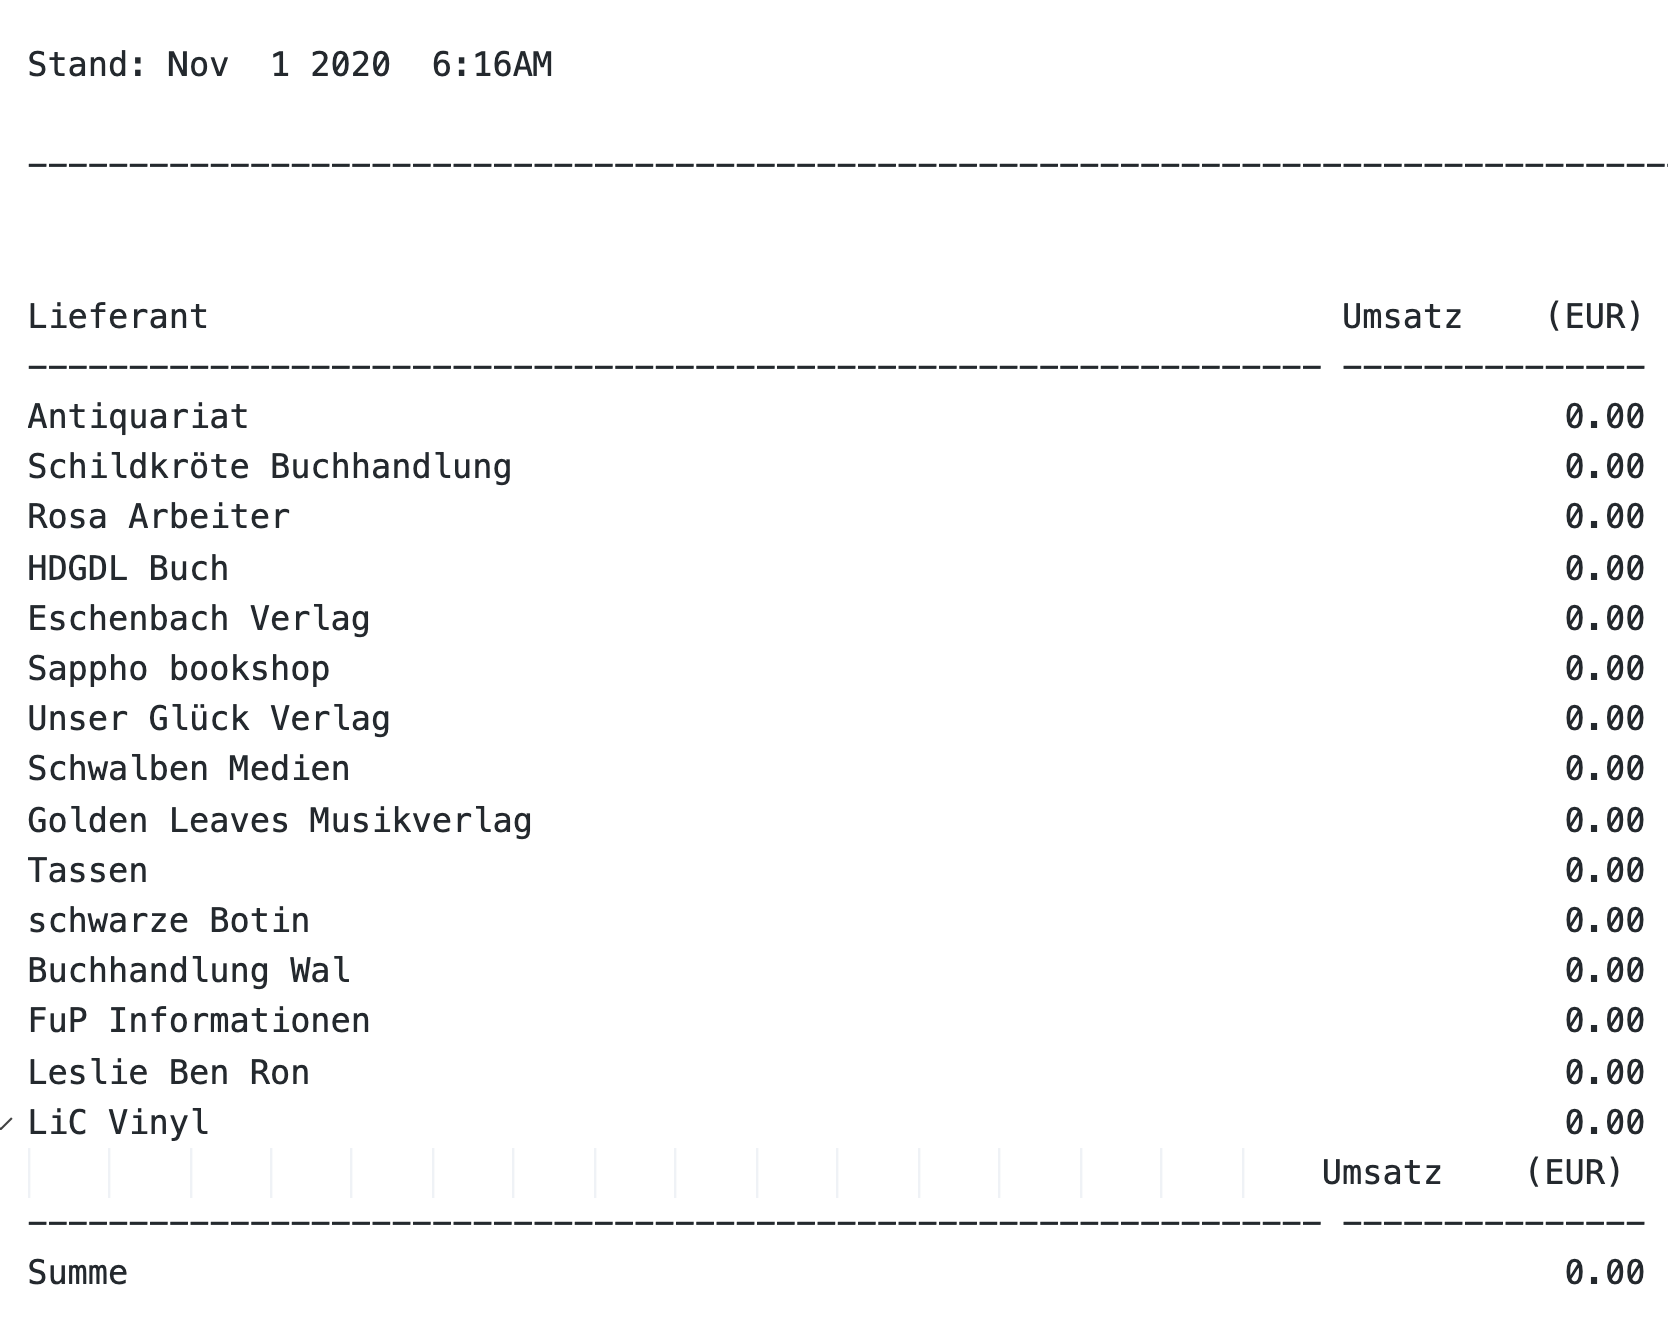
\includegraphics[width=6.5cm, height=7.0cm]{umsatzuebersicht_mtl}
            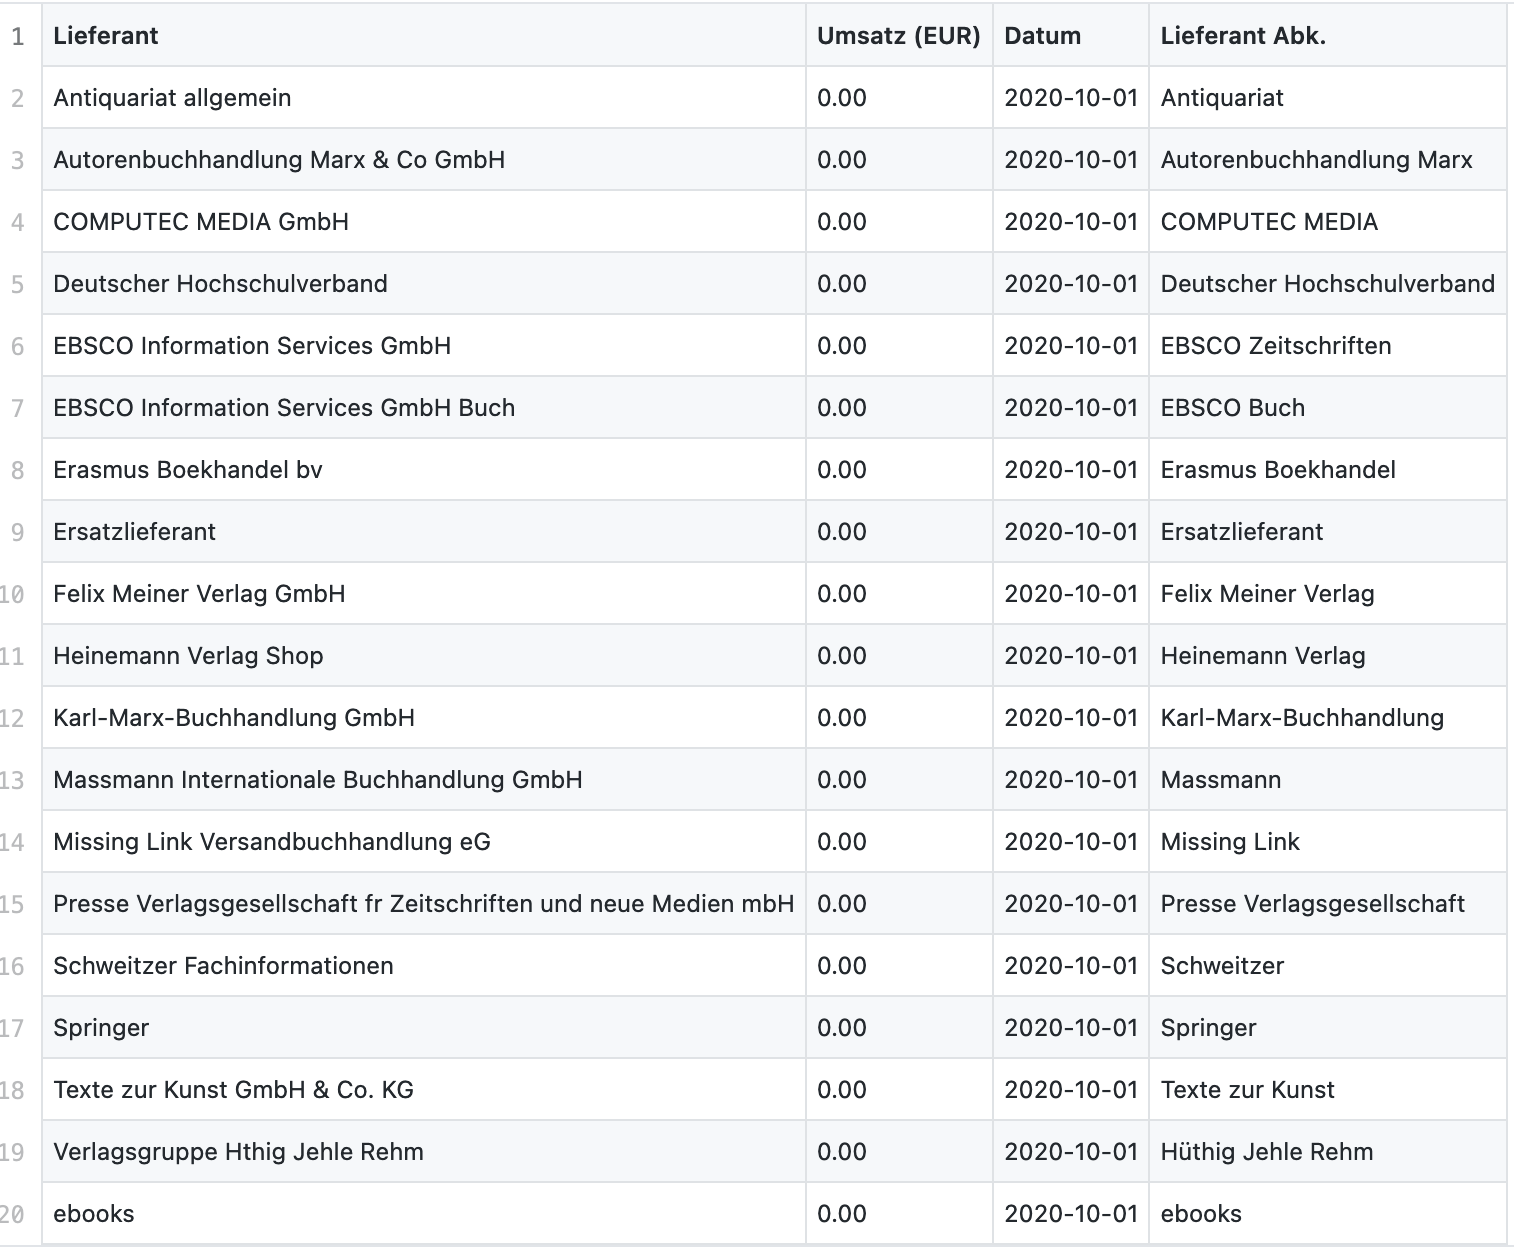
\includegraphics[width=6.5cm, height=7.0cm]{umsatz_csv_bsp}
            \caption{Monatliche Umsatzübersicht nach Ablauf Teilsystem Import}
            \label{fig:umsatzuebersicht_csv}
    \end{figure}


    Die Daten liegen nun in den Speicherverzeichnissen vor und können durch das Teilsystem 2 Datenbearbeitung 
    nun weiterbearbeitet werdenn.
    

    \noindent
    \textit{Teilsystem 2 Datenbearbeitung}

    Das Teilsystem 2 hat als Ziel die Daten für die Darstellung im Dashboard vorzubereiten. Der weitere Zweck dieses
    Teilsystem ist die Vorbereitung der Daten von der Erstellung der Datenvisualisierungen zu trennen. Ein Grund hierfür
    ist, den Programmcode im Teilsystem 3 nicht mit dem Programmcode der Datenmanipulation zu überfrachten. 
    %Ebenfalls haben Überlegungen der Latenzzeit eine Rolle gespielt.
    Deswegen werden in dem Teilsystem Datenbearbeitung Daten mit pandas so bearbeitet, 
    dass entweder Teilmengen der eigentlichen Daten oder Ergebnisse mathematischer Operationen durch das Teilsystem 3 
    zu Datenvisualisierungen nur noch weiterverarbeitet werden müssen. Die Vorbereitung der Daten umfasst einzelne Berechnungen 
    wie \texttt{mean()} oder \texttt{sum()}. Ferner werden im Teilsystem 2 die Sortierung, Gruppierung, Filterung der 
    Daten nach bestimmten Aspekten vollzogen, die in den Anwendungsfällen im \autoref{chap:four_one_five} formuliert sind.
    
    Für das Teilsystem Datenbearbeitung ist das Modul \texttt{data\_prep} zentral. Die Klassenstruktur dieses Moduls ist eine 
    Basisklasse von der vier Kindklassen erben. Es gibt Kindklassen für Umsatz- und Budgetdaten, für Bestands- und Neuerwerbungsdaten, für die Daten der Ausleihe und 
    der Lesesaalnutzung. Aufgrund der ähnlichen Datenstruktur der Umsatz- und Budgetdaten genügt eine Klasse für beide.
    Der Gesamtbestand und die monatlichen Neuerwerbungen berufen sich auf denselben Datenbestand, so dass hier ebenfalls auf eine Aufteilung auf mehrere Klassen verzichtet wurde.
    Für jede Kindklasse wurden Methoden geschrieben, die auf den spezifischen Bibliotheksdaten verschiedene Manipulationen ausführen.
    Die Ergebnisse werden von jeder Methode zurückgeben. \autoref{fig:classes data_prep} zeigt die Basisklasse und die vier Kindklassen mit ihren Methoden.


    \begin{figure}[H]
        \centering
            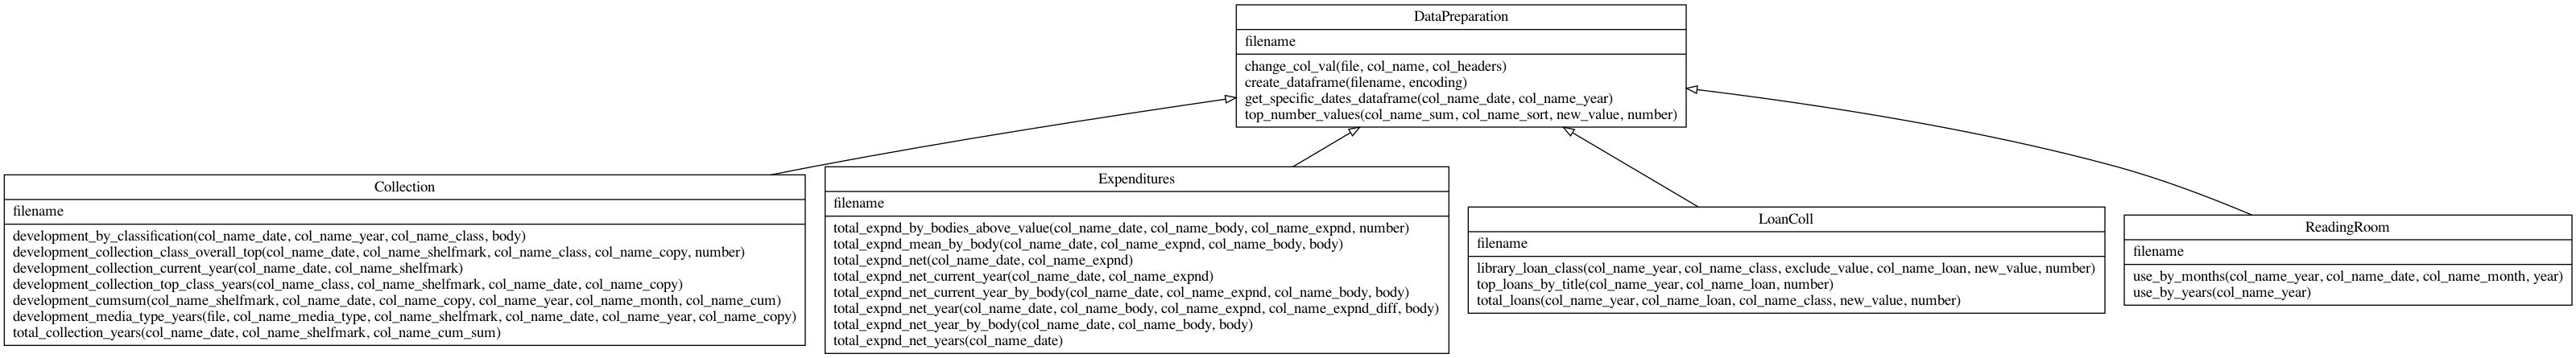
\includegraphics[width=15cm, height=5.5cm]{data_prep}
            \caption{Klassendiagramm - Teilsystem Datenbearbeitung}
            \label{fig:classes data_prep}
    \end{figure}

    Der Ablauf innerhalb des Teilsystems besteht aus zwei Schritten.\\
    (1) Das Laden der einzelnen csv-Dateien in dem pandas Dataframe aus dem Zielverzeichnis wird durch die Methode \texttt{create\_dataframe()} der Basisklasse geregelt.
    %Es wird noch einmal sichergestellt, dass die Daten in einem Zeichenformat wie utf-8 in das pandas Dataframe geladen werden.
    Beim Aufrufen des Konstruktor beziehungsweise der \texttt{init}-Methode der Klasse wird die Methode \texttt{create\_dataframe} 
    automatisch mit aufgerufen. Da die Methode und die Konstruktor-Properties der Basisklasse an die Kindklassen vererbt werden, kann in den Kindklassen das Objekt ebenfalls mit dem 
    pandas Dataframe initiiert werden. Die Objekte werden im nächsten Schritt durch die spezifischen Methoden der Kindklassen bearbeitet.\\
    (2) Das Ergebnis der Manipulation der pandas Dataframes ist auf die Darstellung der Daten im Dashboard ausgerichtet. Als Input der einzelnen Methoden der
    Kindklassen werden verschiedene Parameter verlangt, mit denen der Dataframe entweder manipuliert oder auf ihm Berechnungen ausgeführt werden können. 
    Um die Daten für das Teilsystem 3 vorzubereiten, können verschiedene Transformationsschritte auf den Daten in den Methoden ausgeführt werden. 
    Die Rückgabewerte der Methoden sind veränderte pandas Dataframes, pandas Series oder einzelne Ergebnisse mathematischer Operationen.
    
    % Bei der folgenden Methode interessieren für die Darstellung im Dashboard nur die Umsatz/Budget-Daten für spezifische Datums-Daten. Hintergrund ist der, dass die 
    % monatlichen Umsatz- und Budgetdaten im Jahr akkumuliert werden. Wenn das Budget und der Umsatz nur Jahresweise dargestellt werden sollen, 
    % interessieren dementsprechend nur die Datensätze jeweils vom Dezember beziehungsweise vom aktuellen Monat im Jahr.
    

    % \begin{lstlisting}[language=Python, caption=Python example]
        
    %     def total_expnd_net_years(self, col_name_date):
    %         ...
    %         self._df = self.get_specific_dates_dataframe(col_name_date)
    %         return self._df

    % \end{lstlisting}
    

    % Die Methode \texttt{total\_expnd\_net\_years} der \texttt{Expenditures}-Klasse gibt nach einem Transformationsschritt einen pandas Dataframe zurück.
    % Der Transformationsschritt beinhaltet die Filterung des Dataframes nach spezifischen Werten in der Spalte des übergebenden Spaltennamens.
    % Zu diesem Zweck wird noch die Methode\\
    % \texttt{get\_specific\_dates\_dataframe} aufgerufen. 
    Anhand der folgenden Methode soll der letzte Schritt verdeutlicht werden.
    Die Methode \texttt{total\_expnd\_net\_current\_year()} der \texttt{Expenditures}-Klasse bestimmt im Allgemeinen die Summe von Werten einer Spalte, gefiltert
    nach einem Wert einer anderen Spalte eines pandas Dataframes. Mit dieser Methode soll so zum Beispiel konkret der Gesamtumsatz des 
    laufenden Jahres bestimmt werden.

    \begin{lstlisting}[language=Python, caption=Beispiel Methode Exenditures class]
    def total_expnd_net_current_year(self, col_name_date, col_name_expnd):
        ... 
        self._date_max = self._df[col_name_date].max()
        self._df = self._df.set_index(col_name_date)
        self._df = self._df.loc[self._date_max]

        return self._df[col_name_expnd].sum()  
    \end{lstlisting}

    Als Input erwartet die Methode in der Methodensignatur zwei Spaltennamen als Parameter: den Namen der Datumspalte \texttt{col\_name\_date} nach der gefiltert wird
    und den Namen der Umsatz-Spalte  \texttt{col\_name\_expnd} auf der die Berechnung stattfindet. Der Transformationsprozess im Methodenkörper teilt sich in drei Schritte auf. Da die monatlichen Umsatzdaten im Jahr als 
    akkumulierte Daten vorliegen, interessieren nur die letzten vorhandenen Datensätze des laufenden Jahres. Deswegen
    wird nach diesen gefiltert und ein Dataframe von diesen erstellt. Dementsprechend wird mit der pandas-Funktion \texttt{max()} 
    der maximale Wert in der Datumsspalte zunächst bestimmt und der Variable \texttt{\_date\_max} zugewiesen. Danach wird die Datumsspalte als Index gesetzt. 
    Im dritten Schritt wird der Dataframe mit den Reihen, die der Variable \texttt{\_date\_max} entsprechen, erstellt. Dies geschieht mit der pandas-Funktion \texttt{.loc}, die
    auf den Index der Reihen des Dataframes zugreift. Zum Schluss wird auf Basis der Umsatz-Spalte des Dataframes die Summe mit der pandas-Funktion \texttt{sum()} berechnet 
    und als Rückgabewert zurückgeliefert. Der Rückgabewert kann nun vom Telsystem 3 Darstellung weiterverarbeitet werden.\\


    \noindent
    \textit{Teilsystem 3 Darstellung}\\
    Für die Erschaffung des Dashboards mit seinen Datenvisualisierungen und Interaktionen ist das Teilsystem Darstellung verantwortlich.
    In ihm werden die Ergebnisse des Teilsystems 2 zu Datenvisualisierungen verarbeitet und die Dashboard-Logik bereitgestellt.
    %In ihm werden die Datenvisualisierungen mit den den Ergebnissen aus dem Teilsystem Datenbearbeitung
    %geschaffen. 
    Dazu werden die Bibliothek Plotly Express für die Datenvisualisierungen und die Bibliothek Dash zur Umsetzung des Dashboards genutzt. 
    
    Die Struktur der Dashboard-App entspricht einem Multi-App-Dashboard.
    Aufgrund der Vielzahl an Datenvisualisierungen wurde sich gegen eine Single-Page-Lösung entschieden. Deswegen besteht das Dashboard
    aus drei einzelnen Tabs, auf die die einzelnen Datenvisualisierungen aufgeteilt sind.
    % Aufgrund der vielen Code-Blöcke tendieren Dashboards-Apps, die mit Dash geschrieben wurden zur Unübersichtlichkeit.
    
    Es gibt verschiedene Möglichkeiten Multi-App-Dashboard-Projekte zu strukturieren. Für das vorliegende Projekt wurde sich für die in 
    \autoref{fig:dash structure} gezeigte Struktur entschieden.

    \begin{figure}[H]
        \centering
            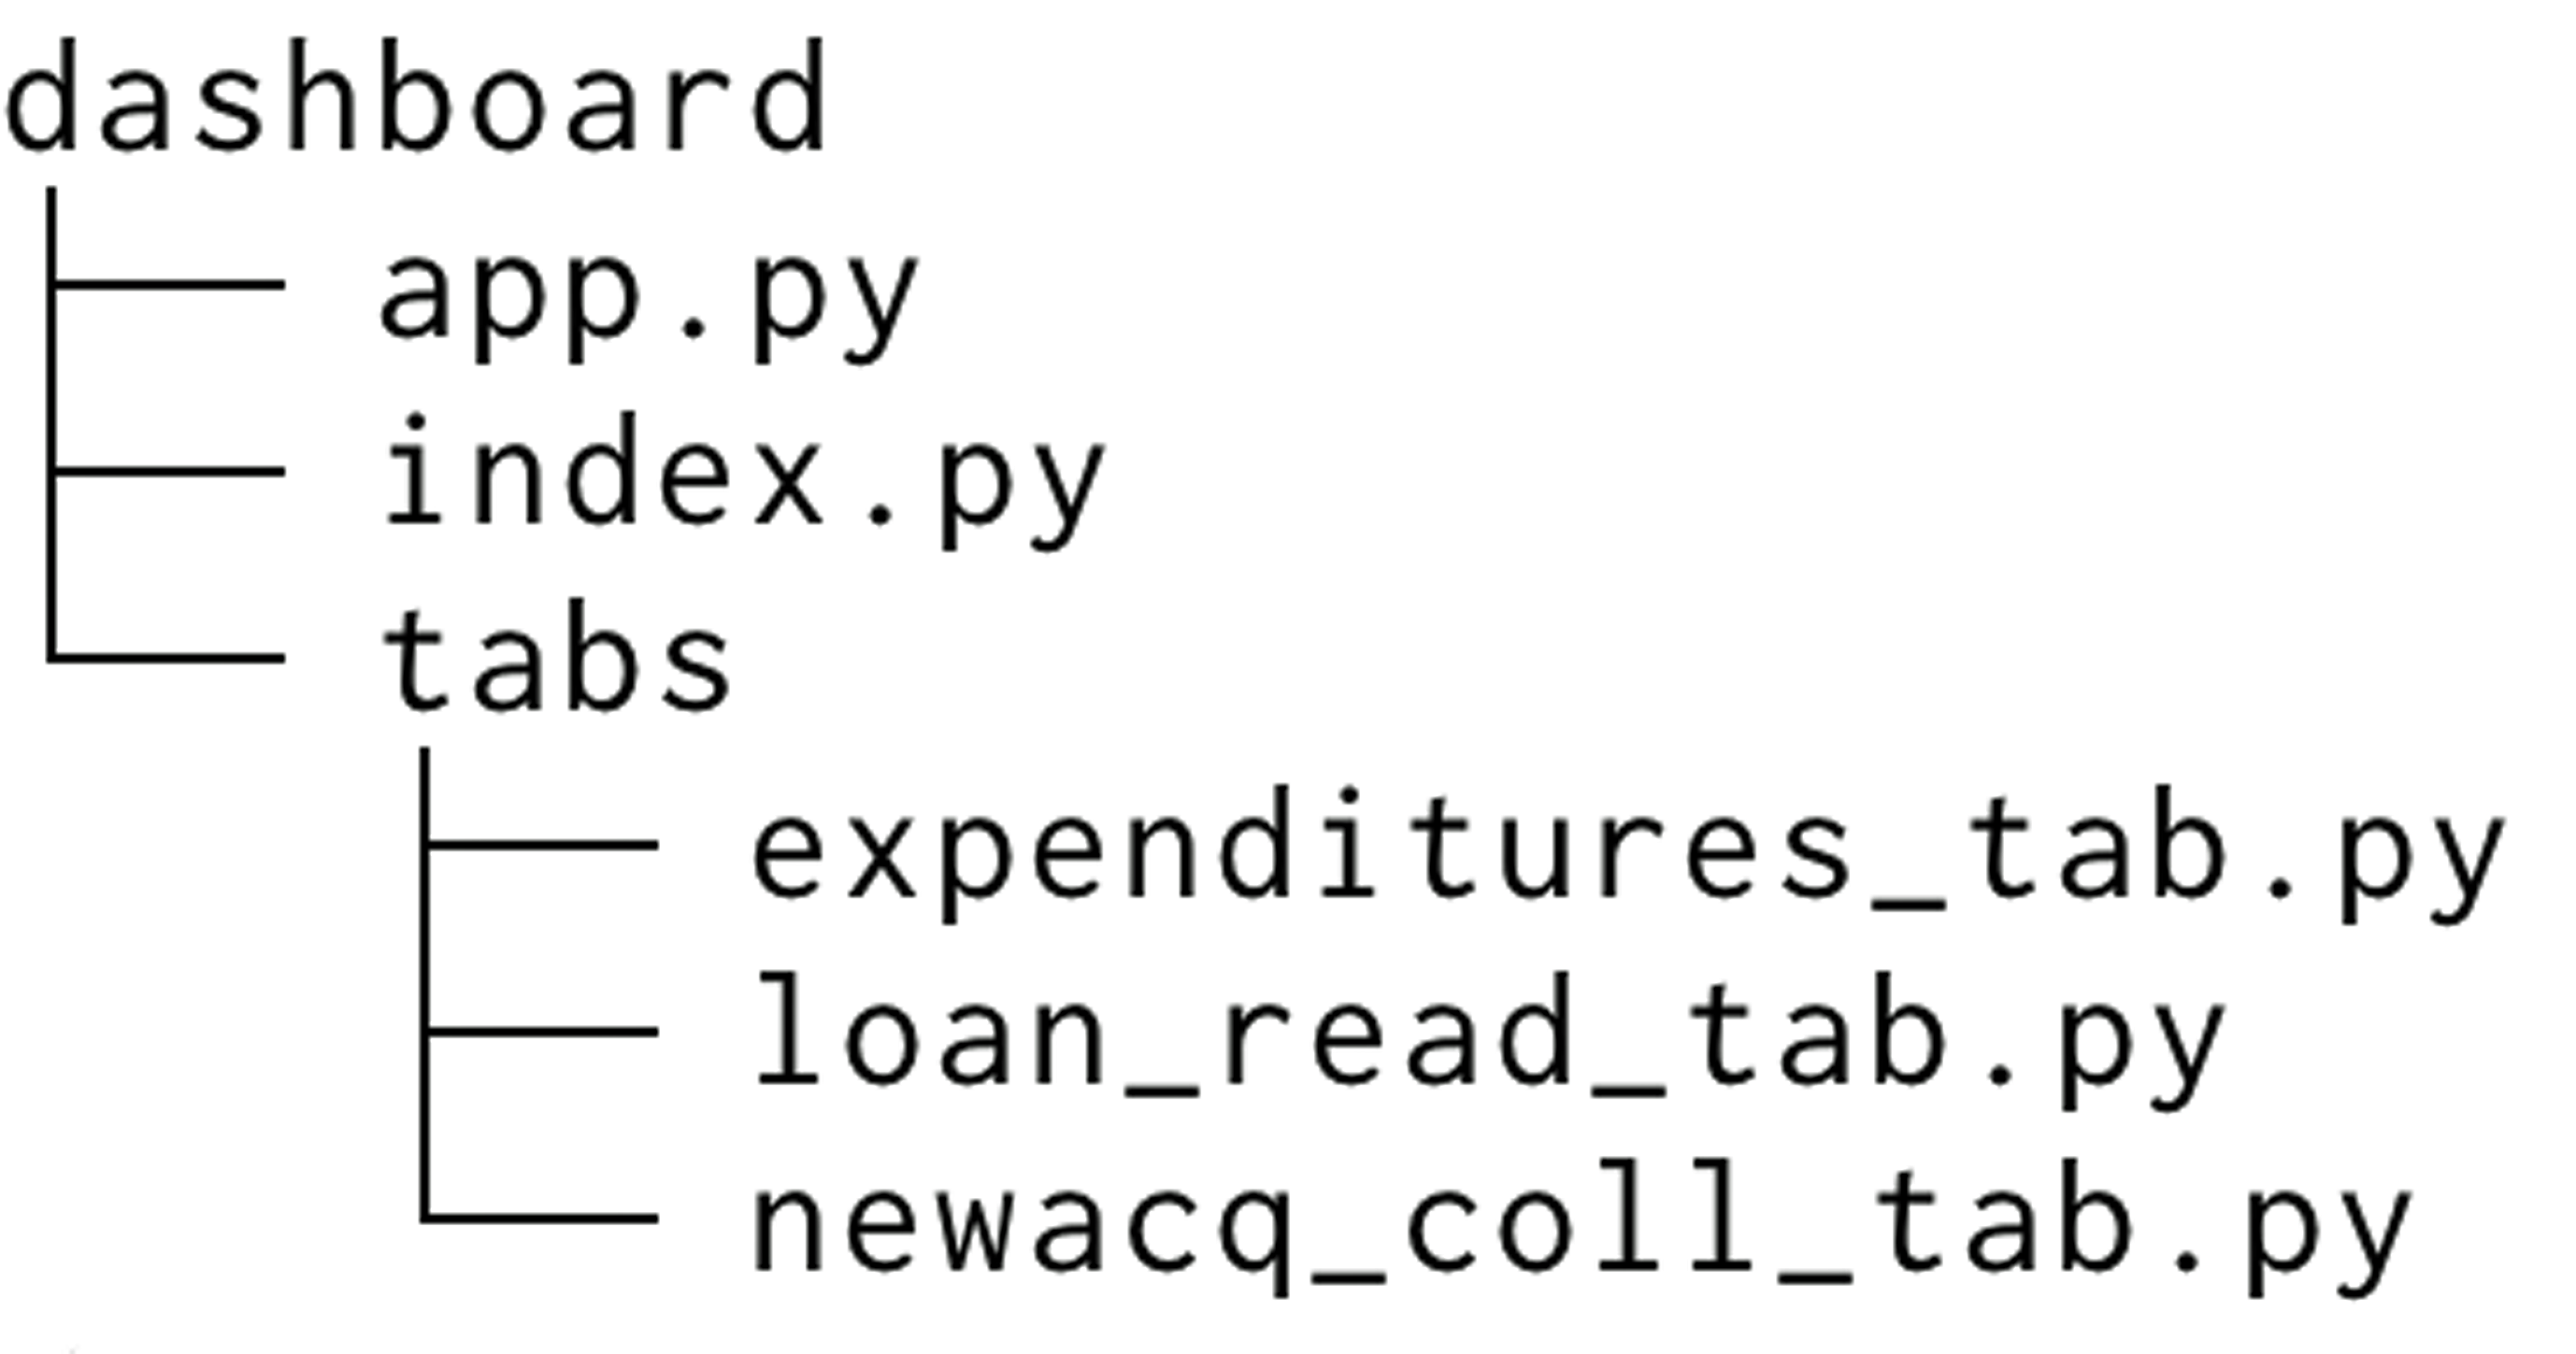
\includegraphics[width=6cm, height=3.5cm]{dash_struc}
            \caption{Struktur Dash Multi-Page App}
            \label{fig:dash structure}
    \end{figure}
    
    Dies ist eine Möglichkeit, wie sie auf der Webseite von Dash für Multi-App-Projekte vorgeschlagen wird \cite[vgl.][]{plotly_url_2021}.
    
    Es wurde versucht, die einzelnen Tabs inhaltlich um bibliothekarische Tätigkeiten zu gruppieren. So werden in der \texttt{expenditures\_app.py}
    Datenvisualisierungen erstellt, die Budget- und die Umsatzdaten visualisieren, während mit Hilfe der \texttt{loan\_read\_app.py}
    Ausleih- und Lesesaalnutzungsdaten dargestellt werden. Mit der \texttt{newacq\_coll\_app.py} wird ermöglicht, Daten aus dem Bereich der Bestandsentwicklung und der 
    Ausleihe zu präsentieren.

    Für jeden Tab gibt es eine separate Datei. Jede einzelne Tab-Datei besteht einerseits aus mehreren Funktionen für die Erschaffung von Datenvisualisierungen der
    Ergebnisse aus Teilsystem 2.\footnote{Zur besseren Lesbarkeit heißt die Gruppe dieser Funktionen im Folgenden \texttt{fig\_data()}.}
    Innerhalb dieser Funktionen werden mit den Plotly-Funktionen \texttt{Plotly Graph Object Figures} geschaffen. 
    Andererseits bestehen die Dateien aus mehreren verschiedenen Funktionen für die Dash-Komponenten wie zum Beispiel Dropdown-Menüs, Cards oder Diagrammen.
    \footnote{Ebenfalls zur besseren Lesbarkeit, heißt die Gruppe dieser Funktionen im Folgenden \texttt{html\_fig()}.}
    Diese Funktionen binden die \texttt{fig\_data()}-Funktionen so ein, dass die \texttt{Plotly Graph Object Figures} im Dashboard zur Anzeige gebracht werden können. 
    Weiterhin sind die \texttt{html\_fig()}-Funktionen zum Teil mit Dekorator-Callback-Funktionen verknüpft, die es ermöglichen mit dem Dashboard zu interagieren. 
    Ferner enthalten die Dateien jeweils eine Layoutfunktion, die das gesamte Layout des
    Tabs bündelt.

    Neben den Funktionen für die Dash-Komponenten und der Datenvisualisierungen, werden in den tab-Dateien noch die benötigten Objekte aus dem Modul \texttt{data\_prep} 
    instantiiert und die Methoden der Kindklassen aus diesem Modul auf diesen angewendet. In der Regel geschieht dies außerhalb der Funktionen.
    Für die Callback-Funktionalität werden aber die Objekte und die Methoden des Moduls \texttt{data\_prep} innerhalb einiger \texttt{html\_fig()} aufgerufen.
    Exemplarisch wird anhand der Erstellung von Plotly Graph Object Figures auf den Aufbau und die Funktionsweise der Funktionen in den Tab-Dateien im Folgenden näher eingegangen.
    \footnote{Auf die Erzeugung von anderen Dash-Elementen wie Cards wird dabei aufgrund der Übersichtlichkeit der Darstellung nicht Bezug genommen. Diesem liegt ein ähnlicher Prozess
    zu Grunde. Es werden aus den berechneten Ergebnissen der Objekte direkt Dash-Komponenten mit Hilfe der \texttt{dash\_bootstrap\_components} erstellt.}
    
    Schematisch zeigt die \autoref{fig:process tab} die Ablauflogik in den Tab-Dateien ohne die callback-Funktionen.
    Die Objekte werden zunächst in Plotly Graph Objects umgewandelt. Diese wiederum werden in Dash-Objekte transformiert und diese werden 
    letztlich in einem Tab-Layout zusammengefasst.
    
    \begin{figure}[H]
        \centering
            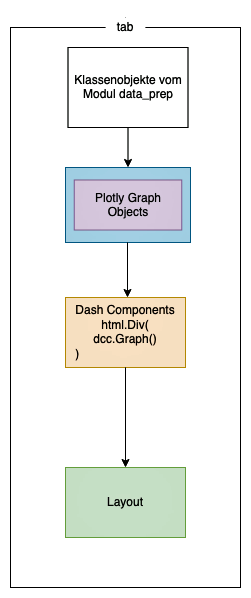
\includegraphics[width=6cm, height=8cm]{ablauf_dash_ohne_cb}
            \caption{Ablauf Tab}
            \label{fig:process tab}
    \end{figure}

    Die grundsätzliche Logik der Funktionsaufrufe sieht in den Tab-Dateien ohne die Callback-Funktionen wie folgt aus:


    \begin{figure}[H]
        \centering
            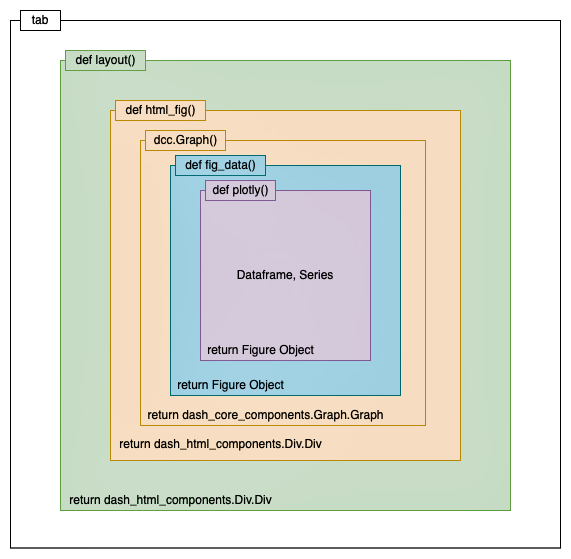
\includegraphics[width=10cm, height=8cm]{funktions_aufrufe_tab}
            \caption{Funktionsaufrufe Tab}
            \label{fig:function call tab}
    \end{figure}

    In der Plotly-Funktion, die das \texttt{Plotly Graph Object Figure} erzeugt, werden die durch die Methoden der Kindklassen bearbeiteten Objekte (Dataframes, Series) 
    als Parameter entgegengenommen. Zusätzlich müssen noch weitere Parameter übergeben werden, die für die jeweiligen Diagrammtypen wichtig sind.
    Andere Parameter, die das Layout festlegen, sind dagegen optional \cite[vgl.][]{plotly_plotlygraph_objectsbar_2021}.
    
    Im folgenden Beispiel wird in der Funktion \texttt{fig\_total\_expnd()} aus \texttt{expenditures\_app.py} ein horizontal gekipptes Figure-Objekt
    mit dem pandas Dataframe \texttt{df\_total\_expnd} durch den Aufruf der Plotly-Funktion \texttt{bar()} erstellt. 
    Es werden zusätzlich in dem Funktionsaufruf noch die x-Achse und y-Achse mit den Werten der Spalten 'Umsatz (EUR)' und 'Datum' festgelegt. 

    \begin{lstlisting}[language=Python, caption=Funktion fig\_total\_expnd() Auszug 1]
    def fig_total_expnd():
        ...
        fig = px.bar(df_total_expnd,
            x='Umsatz (EUR)',
            y='Datum',
            orientation='h',
            ...
        )
        ...
    \end{lstlisting}
    
    Weitere Funktionen von Plotly Express bearbeiten die \texttt{Plotly Graph Object Figures} in den \texttt{fig\_data()}-Funktionen. 
    So kann durch die \texttt{update\_layout}-Funktion unter anderem der Achsentitel, die Höhe und die Breite der Datenvisualisierung 
    festgelegt werden. Als Rückgabewert der Funktionen \texttt{fig\_data()} werden die \texttt{Plotly Graph Object Figures} zurückgegeben.

    \begin{lstlisting}[language=Python, caption=fig\_total\_expnd() Auszug 2]  
    def fig_total_expnd():
        ...
        fig.update_layout(title_x=0.5,
            xaxis_title='Umsatz in Euro',
            yaxis_title='Jahr',
            height=500)
        fig.update_xaxes(nticks=20)         
        return fig
    \end{lstlisting}

    In dem Beispiel werden der Titel der x- und y-Achse, sowie die
    Größe des Diagramm-Objektes festgelegt. Schließlich wird noch die x-Achse mit der Funktion \texttt{update\_xaxes()} skaliert.
    
    Die \texttt{fig\_data()}-Funktionen werden durch die Graph-Komponente der \texttt{dash\_core\_components} innerhalb der 
    \texttt{html\_fig()}-Funktionen aufgerufen. Diese Komponente ist für die Umsetzung der interaktiven Datenvisualisierungen 
    zuständig. Ebenfalls kann von der Graph-Komponente eine \texttt{id} als Parameter entgegengenommen werden. 
    Diese ist unter anderem wichtig für die eindeutige Adressierung durch die Callback-Funktionen.
    Zudem werden in den \texttt{html\_fig()}-Funktionen durch die \texttt{dash\_html\_components} die Eigenschaften und 
    das Aussehen der Div-Objekte definiert. 
    Dabei werden die Properties unter anderem in der externen css-Datei \texttt{layout.css} definiert, die in dem Verzeichnis \texttt{assets} 
    des Dashboard-Verzeichnisses liegt.

    \begin{lstlisting}[language=Python, caption={html\_fig\_total\_expnd()}] 
        def html_fig_total_expnd():
        ...
        return html.Div(
            [
                html.Div(
                    [
                        dcc.Graph(
                            id='gesamtumsatz',
                            figure=fig_total_expnd()
                        ),
                    ], className="six columns chart_div", style={'margin-top': '20px', 'margin-left': '10px'}
                ),
            ]
        )
        \end{lstlisting}
    
    Die \texttt{html\_fig()}-Funktionen werden schließlich in einer Layoutfunktion eingebunden, die alle Funktionen dieser Art
    für das Gesamtlayout des Tab bündelt. Als Rückgabewert returniert sie ebenso wie die \texttt{html\_fig()}-Funktionen ein Div-Objekt der \texttt{dash\_html\_components}.


    Die Callback-Funktionen wurden für zwei Dropdown-Menüs in zwei Tab-Dateien implementiert.
    Die Werte der Dropdown-Menüs werden aus den uniquen Werten einer Dataframespalte erstellt.
    Der Callback ist als Dekorator für jeweils eine Funktion implementiert. 
    In der Implementierung wird ein Callback ausgelöst, wenn ein Wert über das Dropdown-Menü ausgewählt wird.
    Folgendermaßen wird das im Programmcode für ein Diagramm der Lesesaalnutzung in der \texttt{loan\_read\_app.py} umgesetzt.

    \begin{lstlisting}[language=Python, caption={html\_fig\_total\_expnd()}]        
    
    @app.callback(
    Output(component_id='use_by_month', component_property='figure'),
    [Input(component_id='my-id2', component_property='value')])
    def update_output_div(input_value):
    ...
    return fig_use_by_month(input_value)
    \end{lstlisting}

    % Die Funktionsweise der Callback-Funktionen zeigt die \autoref{fig:process tab_dash_cb}.

    % \begin{figure}[H]
    %     \centering
    %         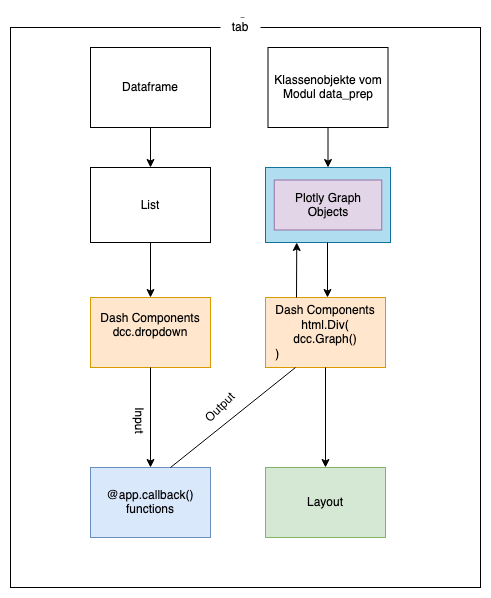
\includegraphics[width=8cm, height=10cm]{ablauf_dash_mit_cb}
    %         \caption{Ablauf Tab mit Callback}
    %         \label{fig:process tab_dash_cb}
    % \end{figure}
 
    Der Callback übergibt den Wert (input\_value) des Dropdown-Menüs an die Funktion \texttt{update\_output\_div()}. 
    Die Funktion gibt das Ergebnis einer \texttt{fig\_data()}-Funktion mit diesem Wert als Argument zurück.
    \footnote{Diese Funktionen übergeben den Methoden der Kindklassen aus dem Modul \texttt{data\_prep} das Argument. 
    Diese erzeugen einen Dataframe basierend auf den übergebenden Argument und geben mit Hilfe der Plotly-Funktionen ein \texttt{Plotly Graph Object Figure} der gefilterten Daten zurück.}
    Der Callback \texttt{@app.callback} übergibt das zurückgegebene Ergebnis an die im Output angegebene Komponente.
    
    Input() und Output() nehmen die ID einer Komponente und die Eigenschaft einer Komponente als Argumente entgegen.
    Die Inputkomponente ist in dem Beispiel die Dropdown-Komponente, während die Outputkomponente die dcc.Graph-Komponente der
    \texttt{html\_fig\_use\_by\_month()} darstellt. Beide werden über die eindeutige \texttt{component\_id} adressiert.
    Multiple Inputs and Outputs sind ebenfalls möglich. So sind in der \texttt{expenditures\_app.py}
    jeweils zwei Diagramme und Zahlenwerte für den Umsatz von den Werten einer Dropdown-Liste abhängig.
    % Dabei handelt es sich um Methoden, die die Daten nach einem Wert filtern und die vom Wert der Dropdown-Liste abhängig sind. Deswegen wird bei diesen
    % Plotly-Funktionen in der Tab-Datei der Wert der Dropdown-Liste als Argument mit in die Funktion gegeben.
    In der folgenden Abbildung ist die Ablauflogik in den Tab-Dateien mit der Callback-Funktion zu sehen.

    \begin{figure}[H]
        \centering
            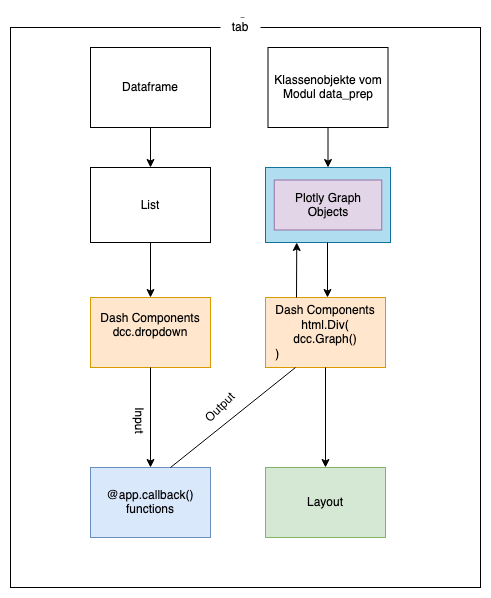
\includegraphics[width=12cm, height=10cm]{ablauf_dash_mit_cb}
            \caption{Ablauf Tab mit Callback}
            \label{fig:process tab_dash_cb}
    \end{figure}


    Zusammengesetzt wird das Layout des Dashboards durch den Aufruf der Layout-Funktion der einzelnden Tab-Dateien in der \texttt{index.py}.
    Die \texttt{index.py} definiert zudem das Layout des gesamten Dashboards. Hier werden auch die Anzahl und die Eigenschaften der Tabs festgelegt. 
    Die Dekorator-Callback-Funktion \texttt{@app.callback()} steuert die Auswahl der Tabs und ruft die jeweiligen Tabs beziehungsweise deren 
    Layouts auf. \autoref{fig:process tab_dash_cb} zeigt im Allgemeinen die Funktionsweise einer Tab-Datei mit der \texttt{index.py}.

    \begin{figure}[H]
        \centering
            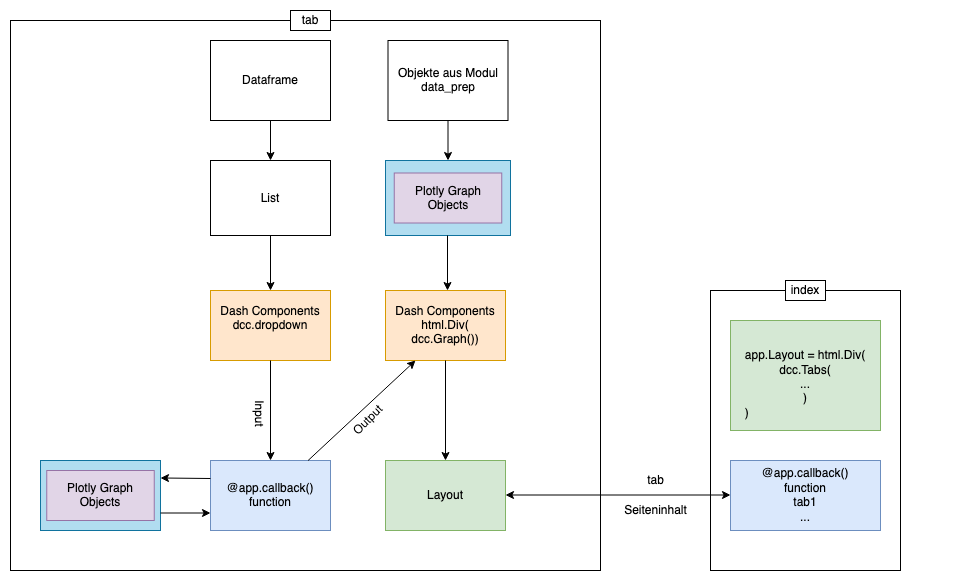
\includegraphics[width=15cm, height=10cm]{ablauf_dash}
            \caption{Ablauf Tab mit index}
            \label{fig:process tab_dash_cb}
    \end{figure}

    Der Einstiegspunkt zur Ausführung des Dashboards ist die Datei \texttt{index.py}. Mit dieser Datei wird das Dashboard mittels \texttt{Flask-Webserver}
    gestartet. Zur Vermeidung zirkulärer Importe ist die Dash-Instanz in der separaten \texttt{app.py} definiert\cite[vgl.][]{plotly_url_2021}.


    %\textit{Standardbericht}\\

\section{Funktionsweise}

    Im Folgenden wird die Funktionsweise des Systems dargelegt. Dabei wird zunächst auf Voraussetzungen eingeganen und dann
    spezifisch auf das Teilsysem 1 Import und der
    praktische Import Daten skizziert. Da die anderen beiden Teilsysteme im Backend angesiedelt sind und keine Schnittstelle
    nach außen bieten, wird auf diese beiden nicht eingegangen. Teilsystem 3 ist soweit von Interesse, da aus diesem das Dashboard
    gestartet wird. Das Dashboard ist die grafische Umsetzung des Teilsysttem2 und 3. Beim Dashboard wird noch kurz auf das Layout
    eingegangen, bevor die Funktionsweise und die Datenvisualisierungen besprochen werden.


    \subsection{Voraussetzungen}
    Der Programmcode zum Projekt liegt auf github. Dort gibt es weitere Informationen zur Installation.
    Das System wurde auf den Betriebssystemen maOS Big Sur, Linux in der Ubuntu-Distribution 20.10. getestet.
    Das Dashboard kann mit auf den aktuellen Versionen der Web-Browser Google Chrome, Firefox und Safari dargestellt werden. 
    Als Minimum an Hardware-Anforderungen wird ein Intel Dual Core i5 (Haswell) mit 8 GB Ram angegeben.
    Mit dem Projekt werden keine bibliothekarischen Daten mitgeliefert.
    \subsection{Daten-Import}
    Der Import der Daten findet über Skripte statt. Diese liegen im Projektverzeichnis \texttt{src/instances}.
    Für Budget, Umsatz, Neuerwerbungen und Ausleihdaten liegen einzelne Python-Skripte bereit, die manuell über die Kommandozeile
    aufgerufen werden können. Zu dem gibt es noch ein shell-Skript, dass die vier Skripte zusammen anstösst. Dieses
    muss ebenfalls manuell aufgerufen werden.
    Nach erfolgreichem Import der Dateien aus den Importverzeichnissen wird eine einfache Erfolgsmeldung auf der Kommandozeile ausgegeben.\footnote{Es gibt Warnungen,
    die angezeigt werden. Diese Warnmeldungen haben keinen Einfluss auf den Import. Im Bearbeitungszeitraum der Arbeit konnte diesen Warnmeldungen leider nicht nachgegangen werden.}

    Die Pfade zu den lokalen Verzeichnissen für Import- und Speichern sind als Konstanten zentral in der configuaration.py 
    im Projektverzeichnis hinterlegt. Dort sind auch noch andere Pfadkonstanten definiert, die auf Look-Up-Dateien verweisen, die das Teilsystem 1
    und das Teilsystem 2 unterstützen. Wichtig ist, dass die zu importierenden Daten über Dateinamen einer gewissen Semantik und 
    über ein gewisses Format verfügen, sonst werden sie nicht importiert (Siehe auch \autoref{chap:five_one_three} Teilsystem 1).

    \subsection{Dashboard}
    Gestartet wird die Dashboard-Application auf der Kommandozeile, in dem \texttt{index.py} im Projektverzeichnis \texttt{dashboard}
    aufgerufen wird. Diese startet den Flask-Webserver mit der Dashboard-App. Der Webserver ist in der \texttt{index.py} so eingestellt, 
    dass er an allen Netzwerkschnittstellen lauscht.


    \begin{figure}[H]
        \centering
            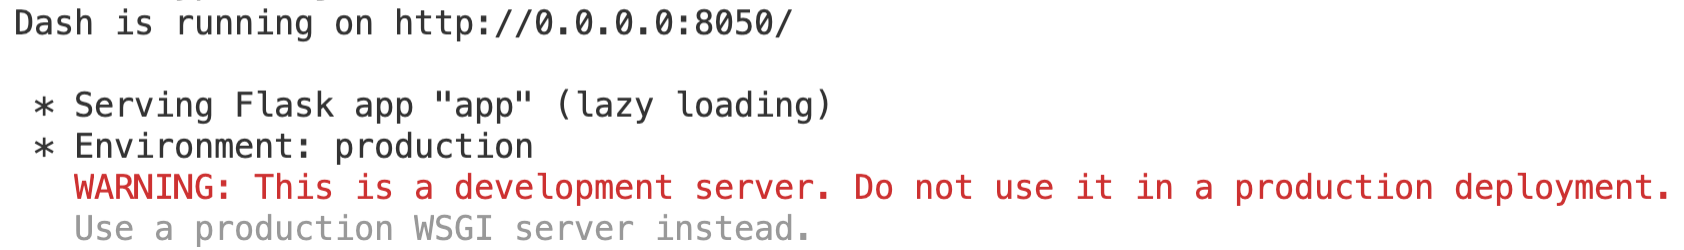
\includegraphics[width=12cm, height=2cm]{flask_webserver}
            \caption{Flask Webserver}
            \label{fig:flask}
    \end{figure}

    Das Dashboard kann mit der angegebenen Adresse vom Web-Browser geöffnet werden.

    Wie im \autoref{chap:five_one_three} Teilsystem 3 beschrieben besteht das Dashboard aus drei Tabs.
    Die Navigation zu den drei Tabs ist im oberen Bereich des Dashboards nebeneinander angeordnet. 
    
    \begin{figure}[H]
        \centering
            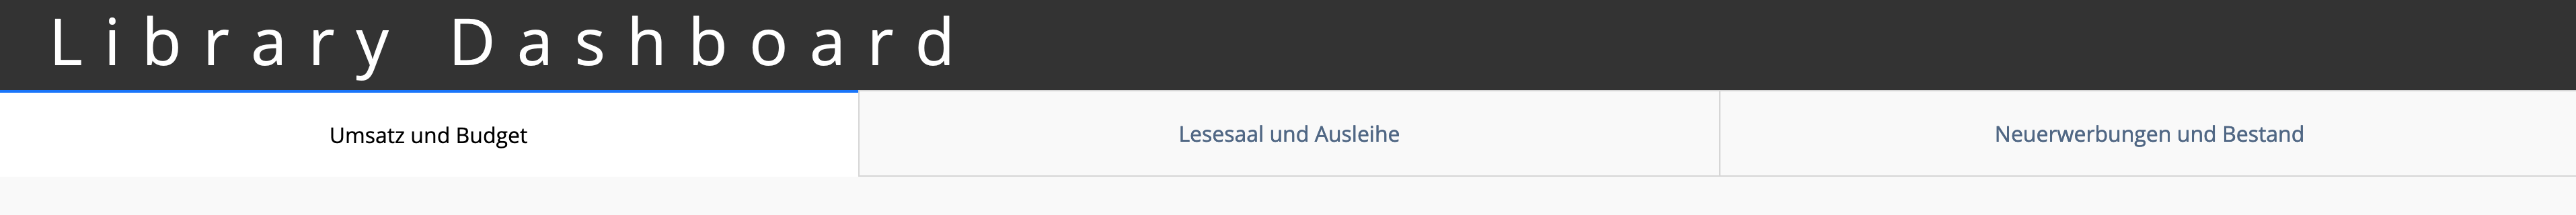
\includegraphics[width=14cm, height=2cm]{tabs}
            \caption{Tabs-Navigation}
            \label{fig:flask}
    \end{figure}

  
    
    Das Layout des Dashboards sieht wie folgt aus:


    Die Tabs des Dashboard bestehen aus verschiedenen Div-Containern, dfdgbsdfg
    
    
    Fast allen Diagrammen wohnt inne, dass man aus der Legende auswählen kann welche Elemente angezeigt bzw. nicht angezeigt werden sollen.
    mitunter auch hover elemente, wenn über die einzelnen Balken oder Linien mit der Maus gefahren 
    

    Nach dem die Adresse Browser geöffnet wurde, wird der Tab \textit{Umsatz und Budget} aufgerufen. Dieser ist
    als default-value im Dashboard-Layout der \texttt{index.py} eingestellt.


    Tab1 - Umsatz und Budget
    
    Bild Tab1
    Was ist dargestellt:

    \begin{figure}[H]
        \centering
            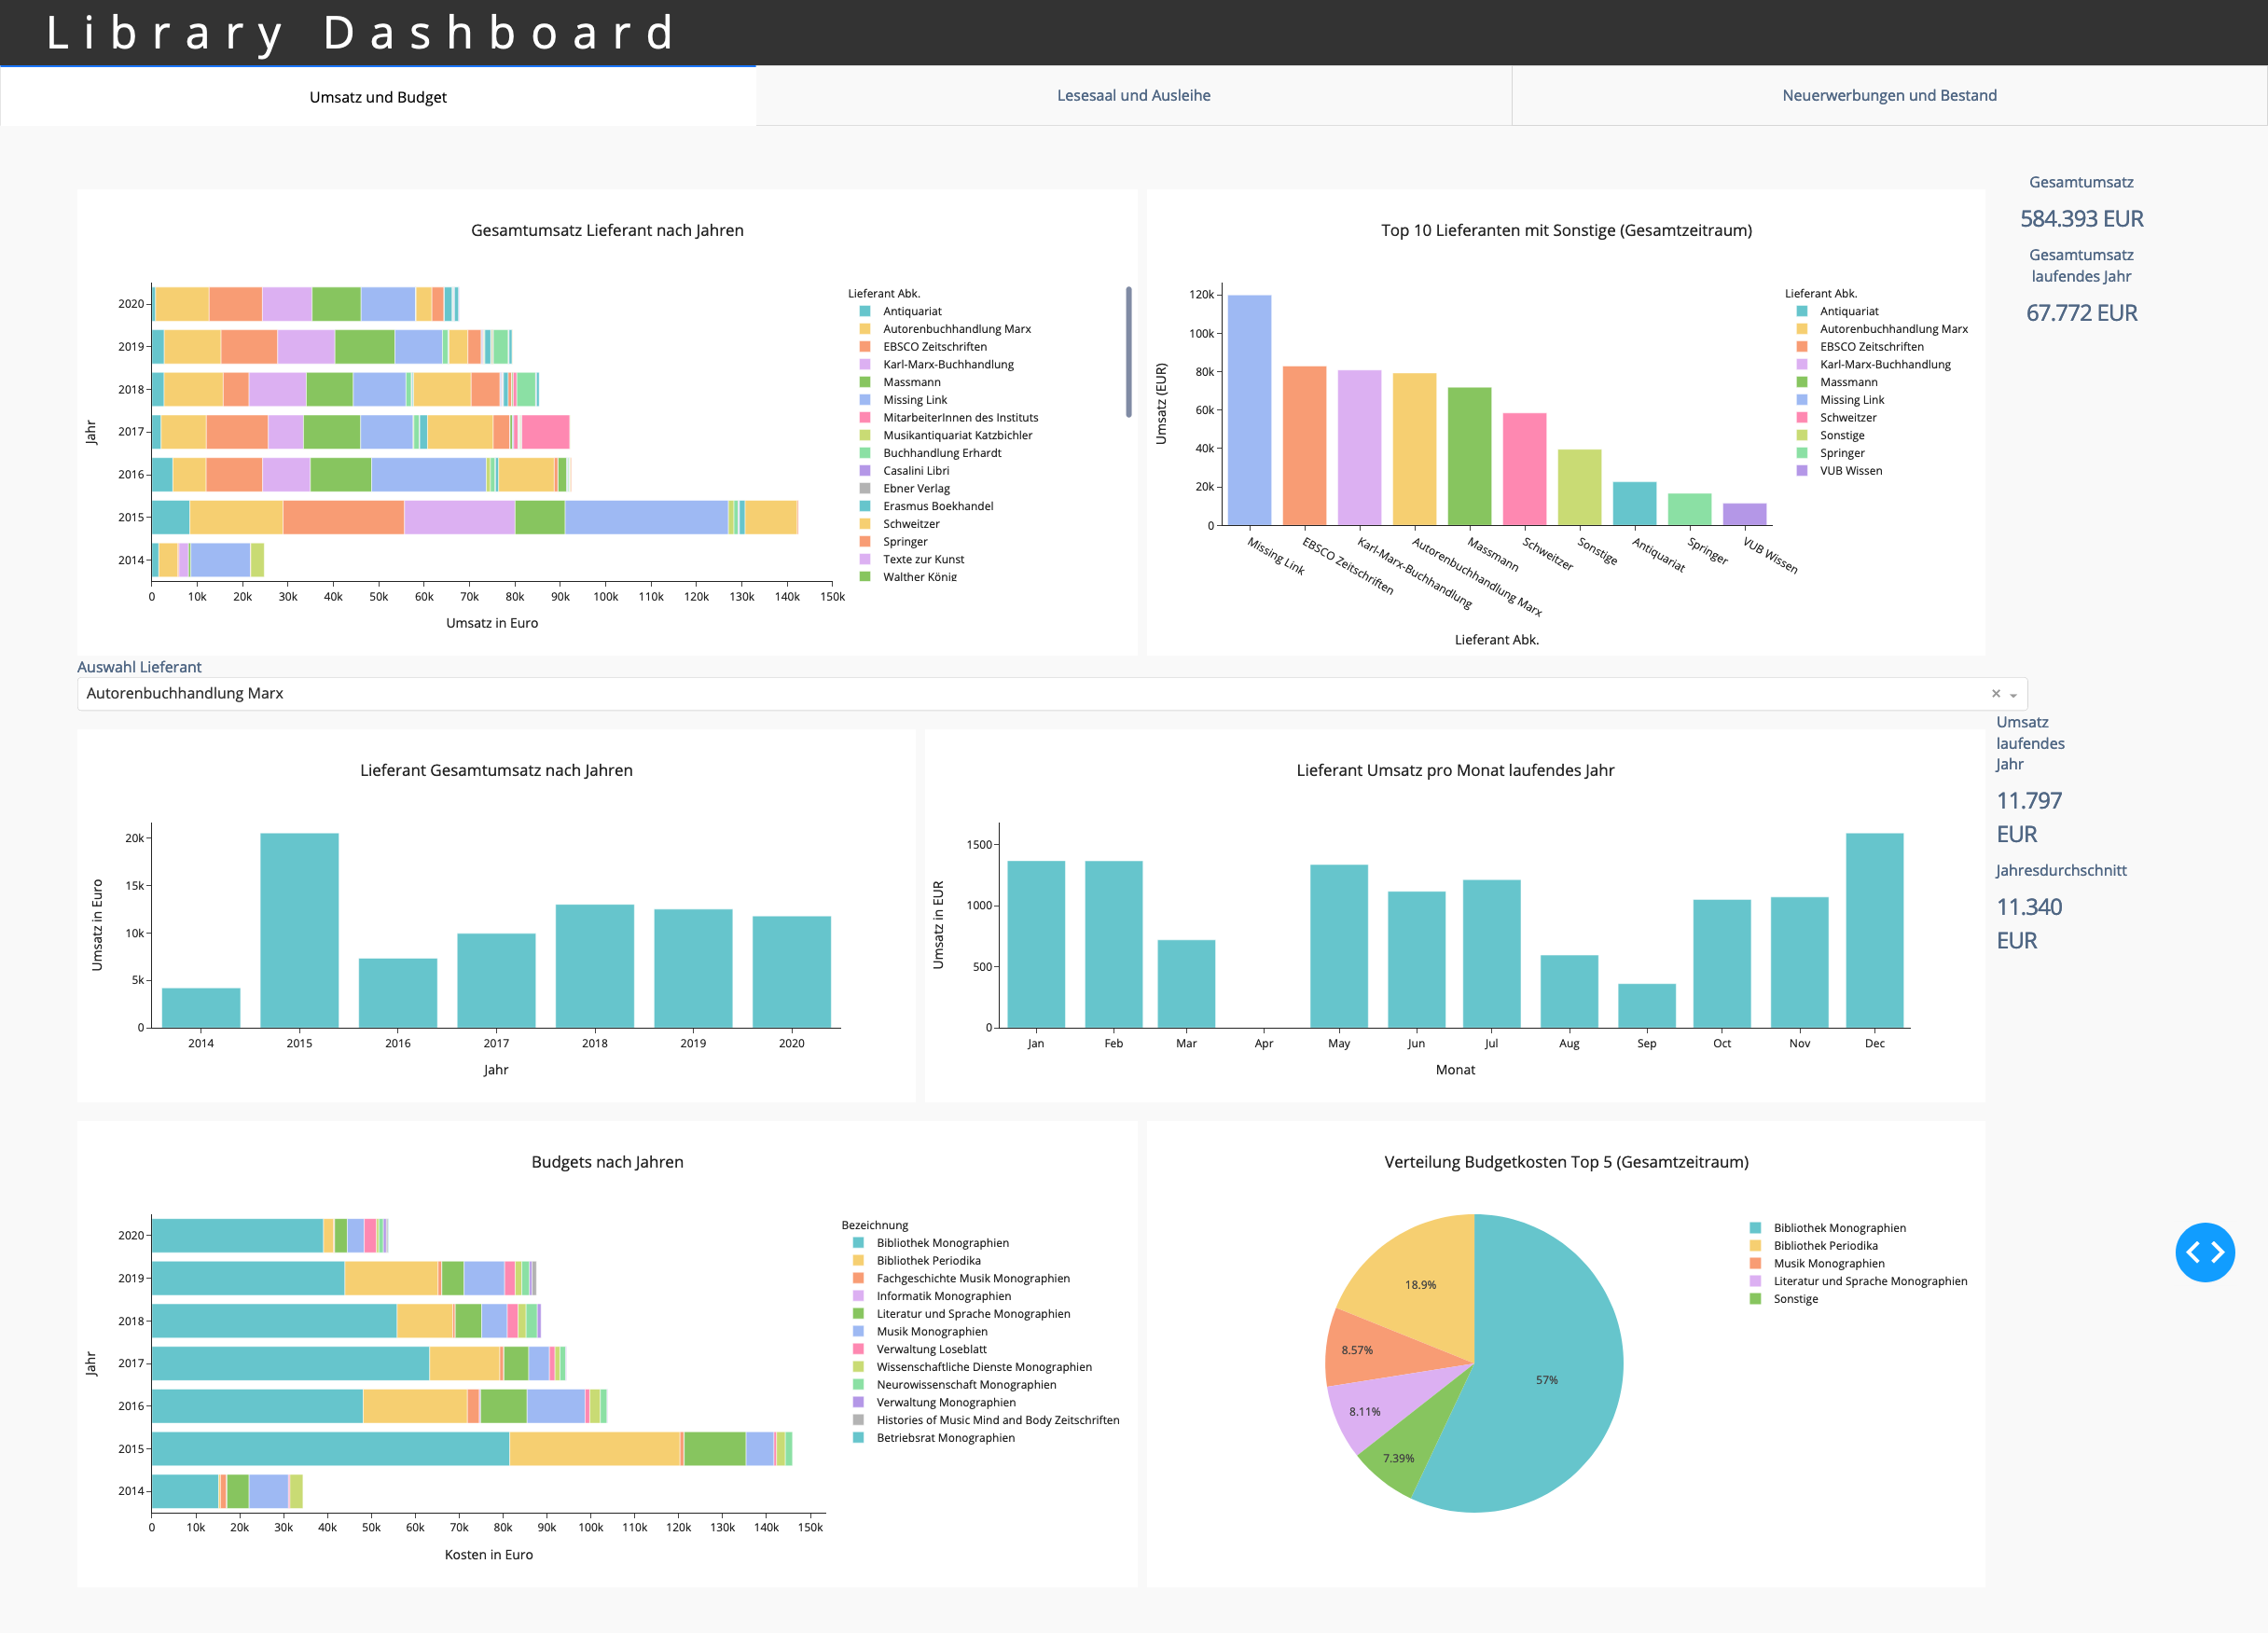
\includegraphics[width=15cm, height=12cm]{tab1}
            \caption{Tab1}
            \label{fig:tab1}
    \end{figure}

    Zu sehen sind sechs Diagramme für die Budget- und Umsatzdaten und 4 Karten-Elemente mit Informationen über den
    Gesamtumsatz und den Lieferanten-Umsatz pro Jahr. 

    zwei Diagramme mit 
        Anzeige des Gesamtumsatz nach Jahren und nach Lieferanten ->  horizontalestapeltes Balkendiagramm
        umsatzstärkste Lieferanten (Top 7) Verteilung in Prozent (Kreisdiagramm)
        
    zwei Diagramme mit interaktiver Auswahl eines Lieferanten über Dropdownmenü
        Anzeige des Gesamtumsatzes nach Jahren für de ausgewählten Lieferanten (Liniendiagramm)
        Anzeige des Umsatzes pro Monat für das laufende Jahr (Balkendiagramm)
    
    zwei Diagramme mit
        Anzeige des Gesamtbudgets nach Jahren und nach Kostenstellen 
        Anzeige kostenintesive (Top 7) Kostenstellen
        
    
    vier Karten mit
        Zahl des Gesamtumsatzes
        Zahl des Umsatzes im Jahr
        Zahl des Umsatzes im laufenden Jahrs für den einzelnen Lieferanten (gekoppelt mit Dropdown-Auswahl)
        Durchschnittlicher Umsatz des Lieferanten (gekoppelt mit Dropdown-Auswahl)
    
    
 
    
    Tab2 - Lesesaal und Ausleihe
    
    \begin{figure}[H]
        \centering
            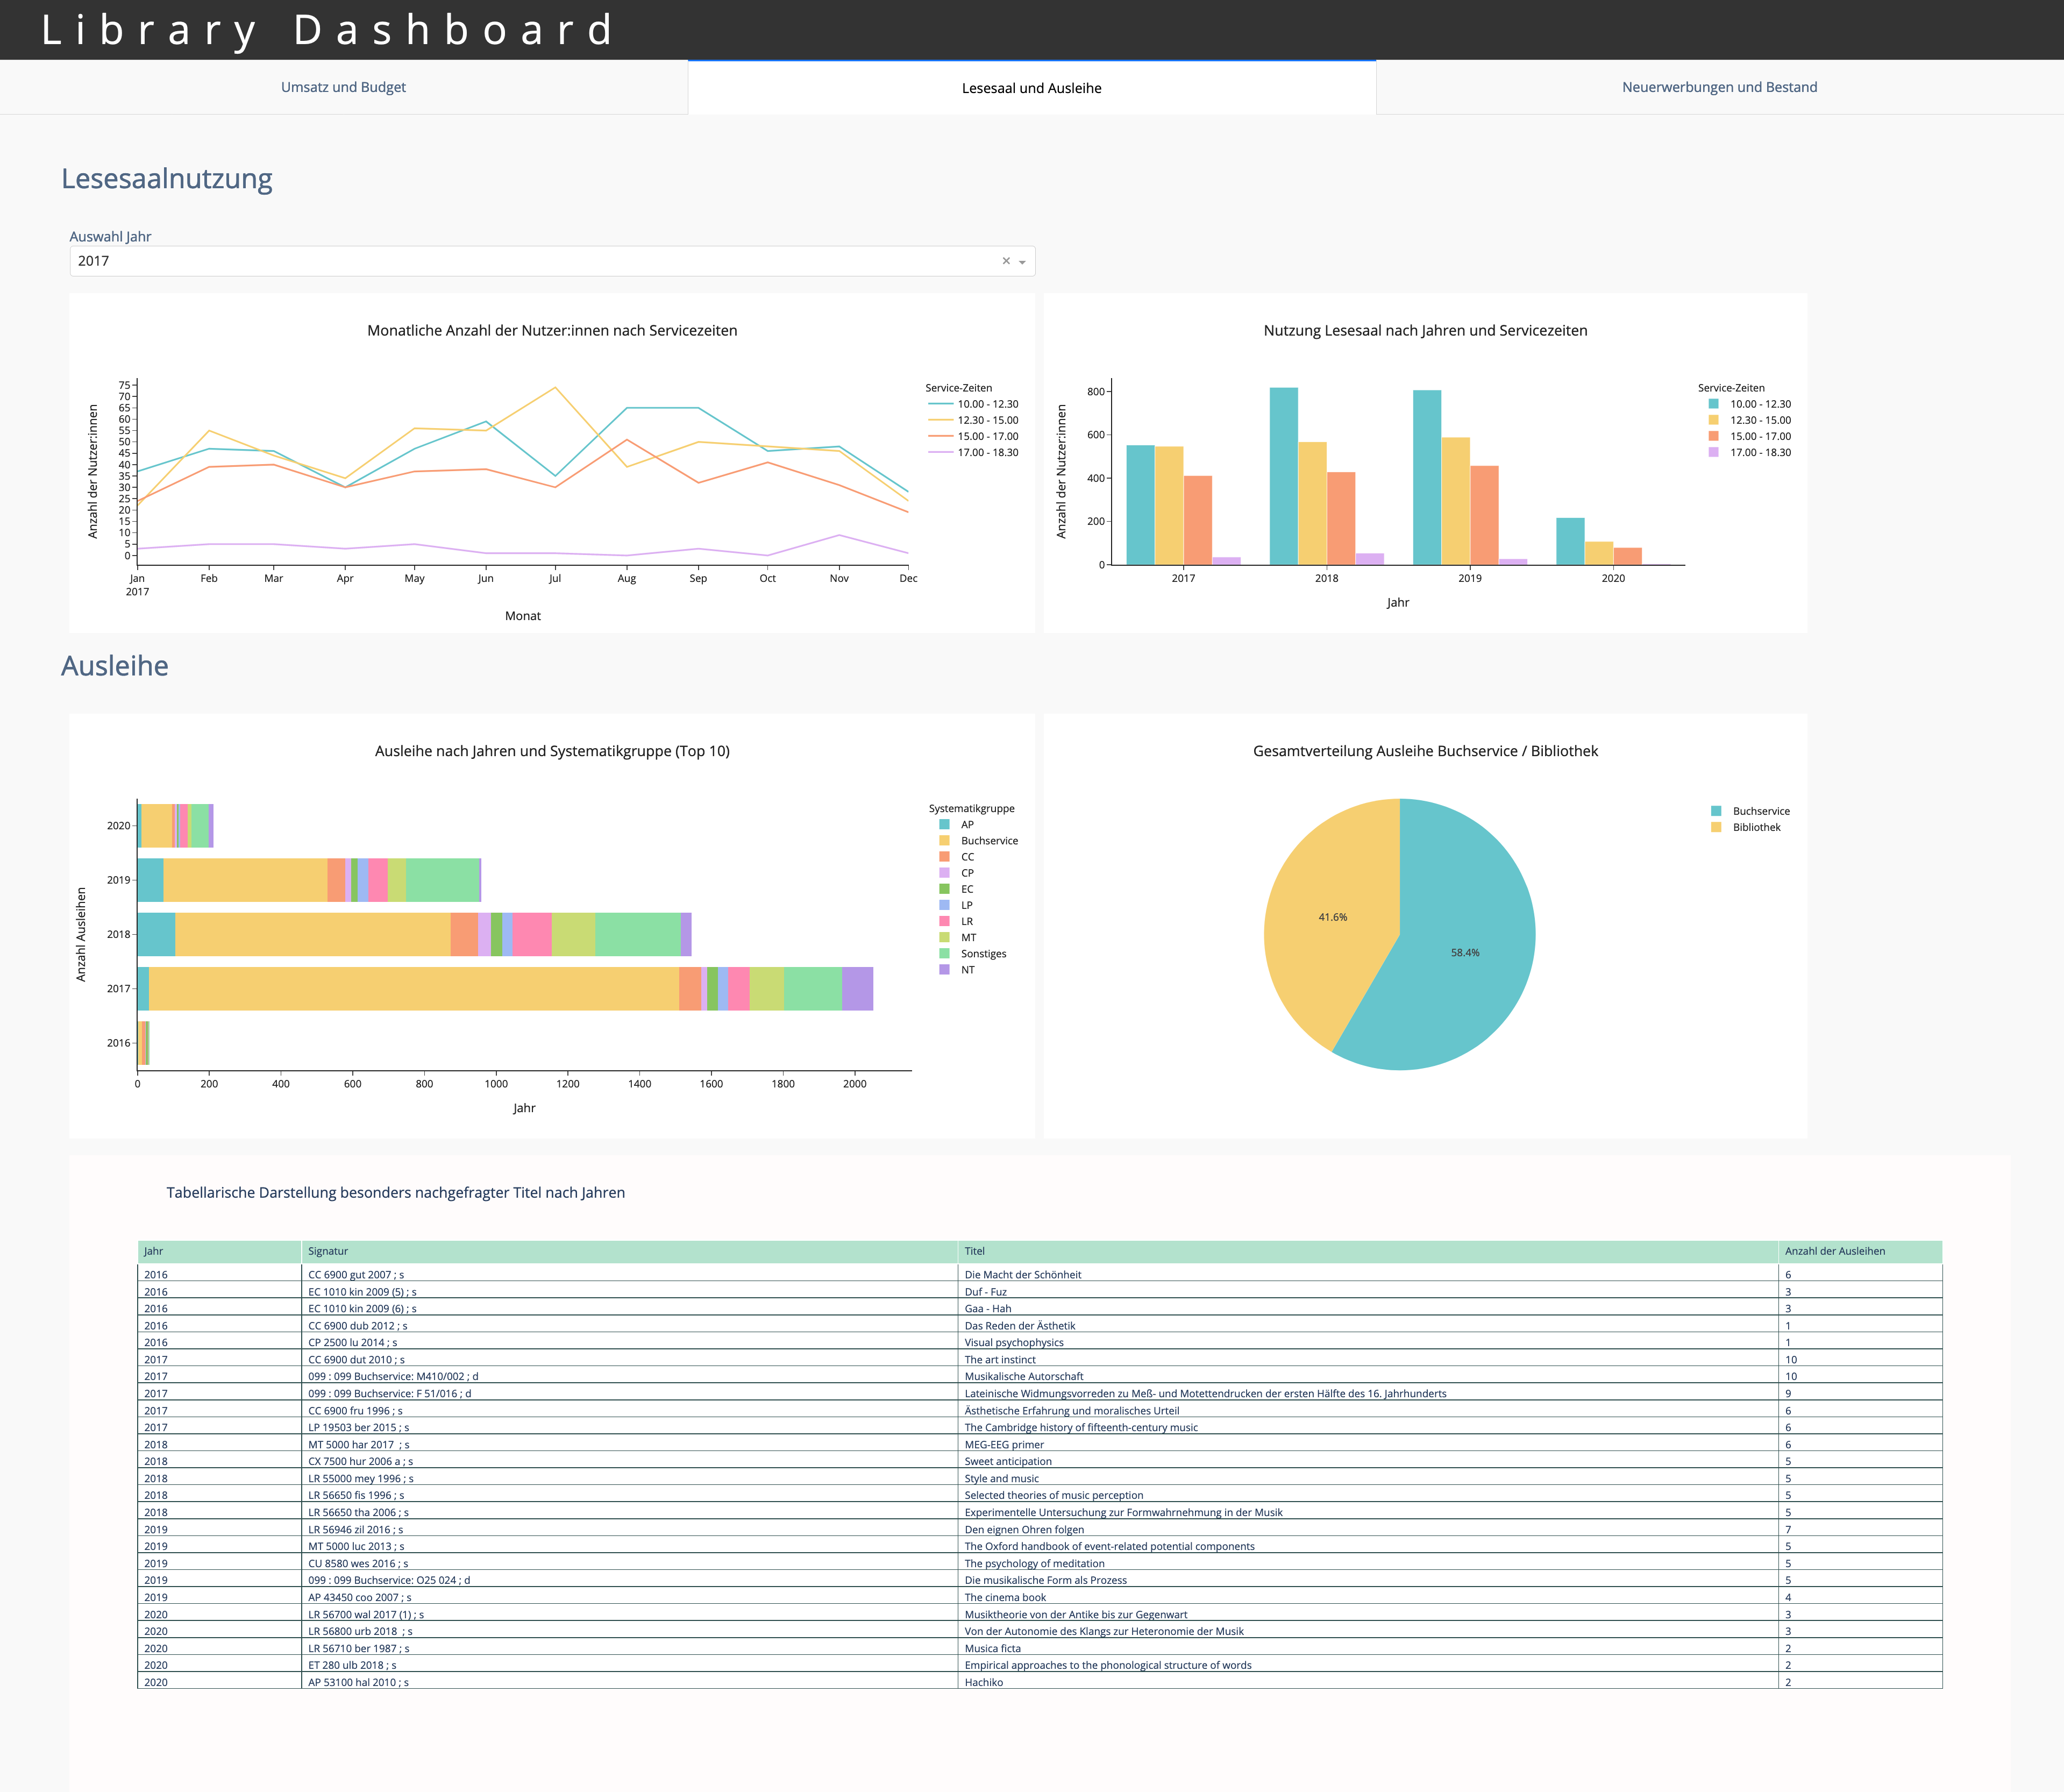
\includegraphics[width=15cm, height=12cm]{tab2}
            \caption{Tab2}
            \label{fig:tab2}
    \end{figure}
    
    zwei Diagramme mit
        Anzeige der Nutzer:innen nach Jahren und nach Service-Zeiten (gruppiertes Balkendiagramm)
        Anzeige der Nutzer:innen nach Monaten und nach Service-Zeiten für das laufende Jahr.
        
     ein Diagramm mit
        Anzeige der Ausleihanzahl nach Jahren (horizontales Balkendiagramm)
    
    Tab3 - Bestand
    
    \begin{figure}[H]
        \centering
            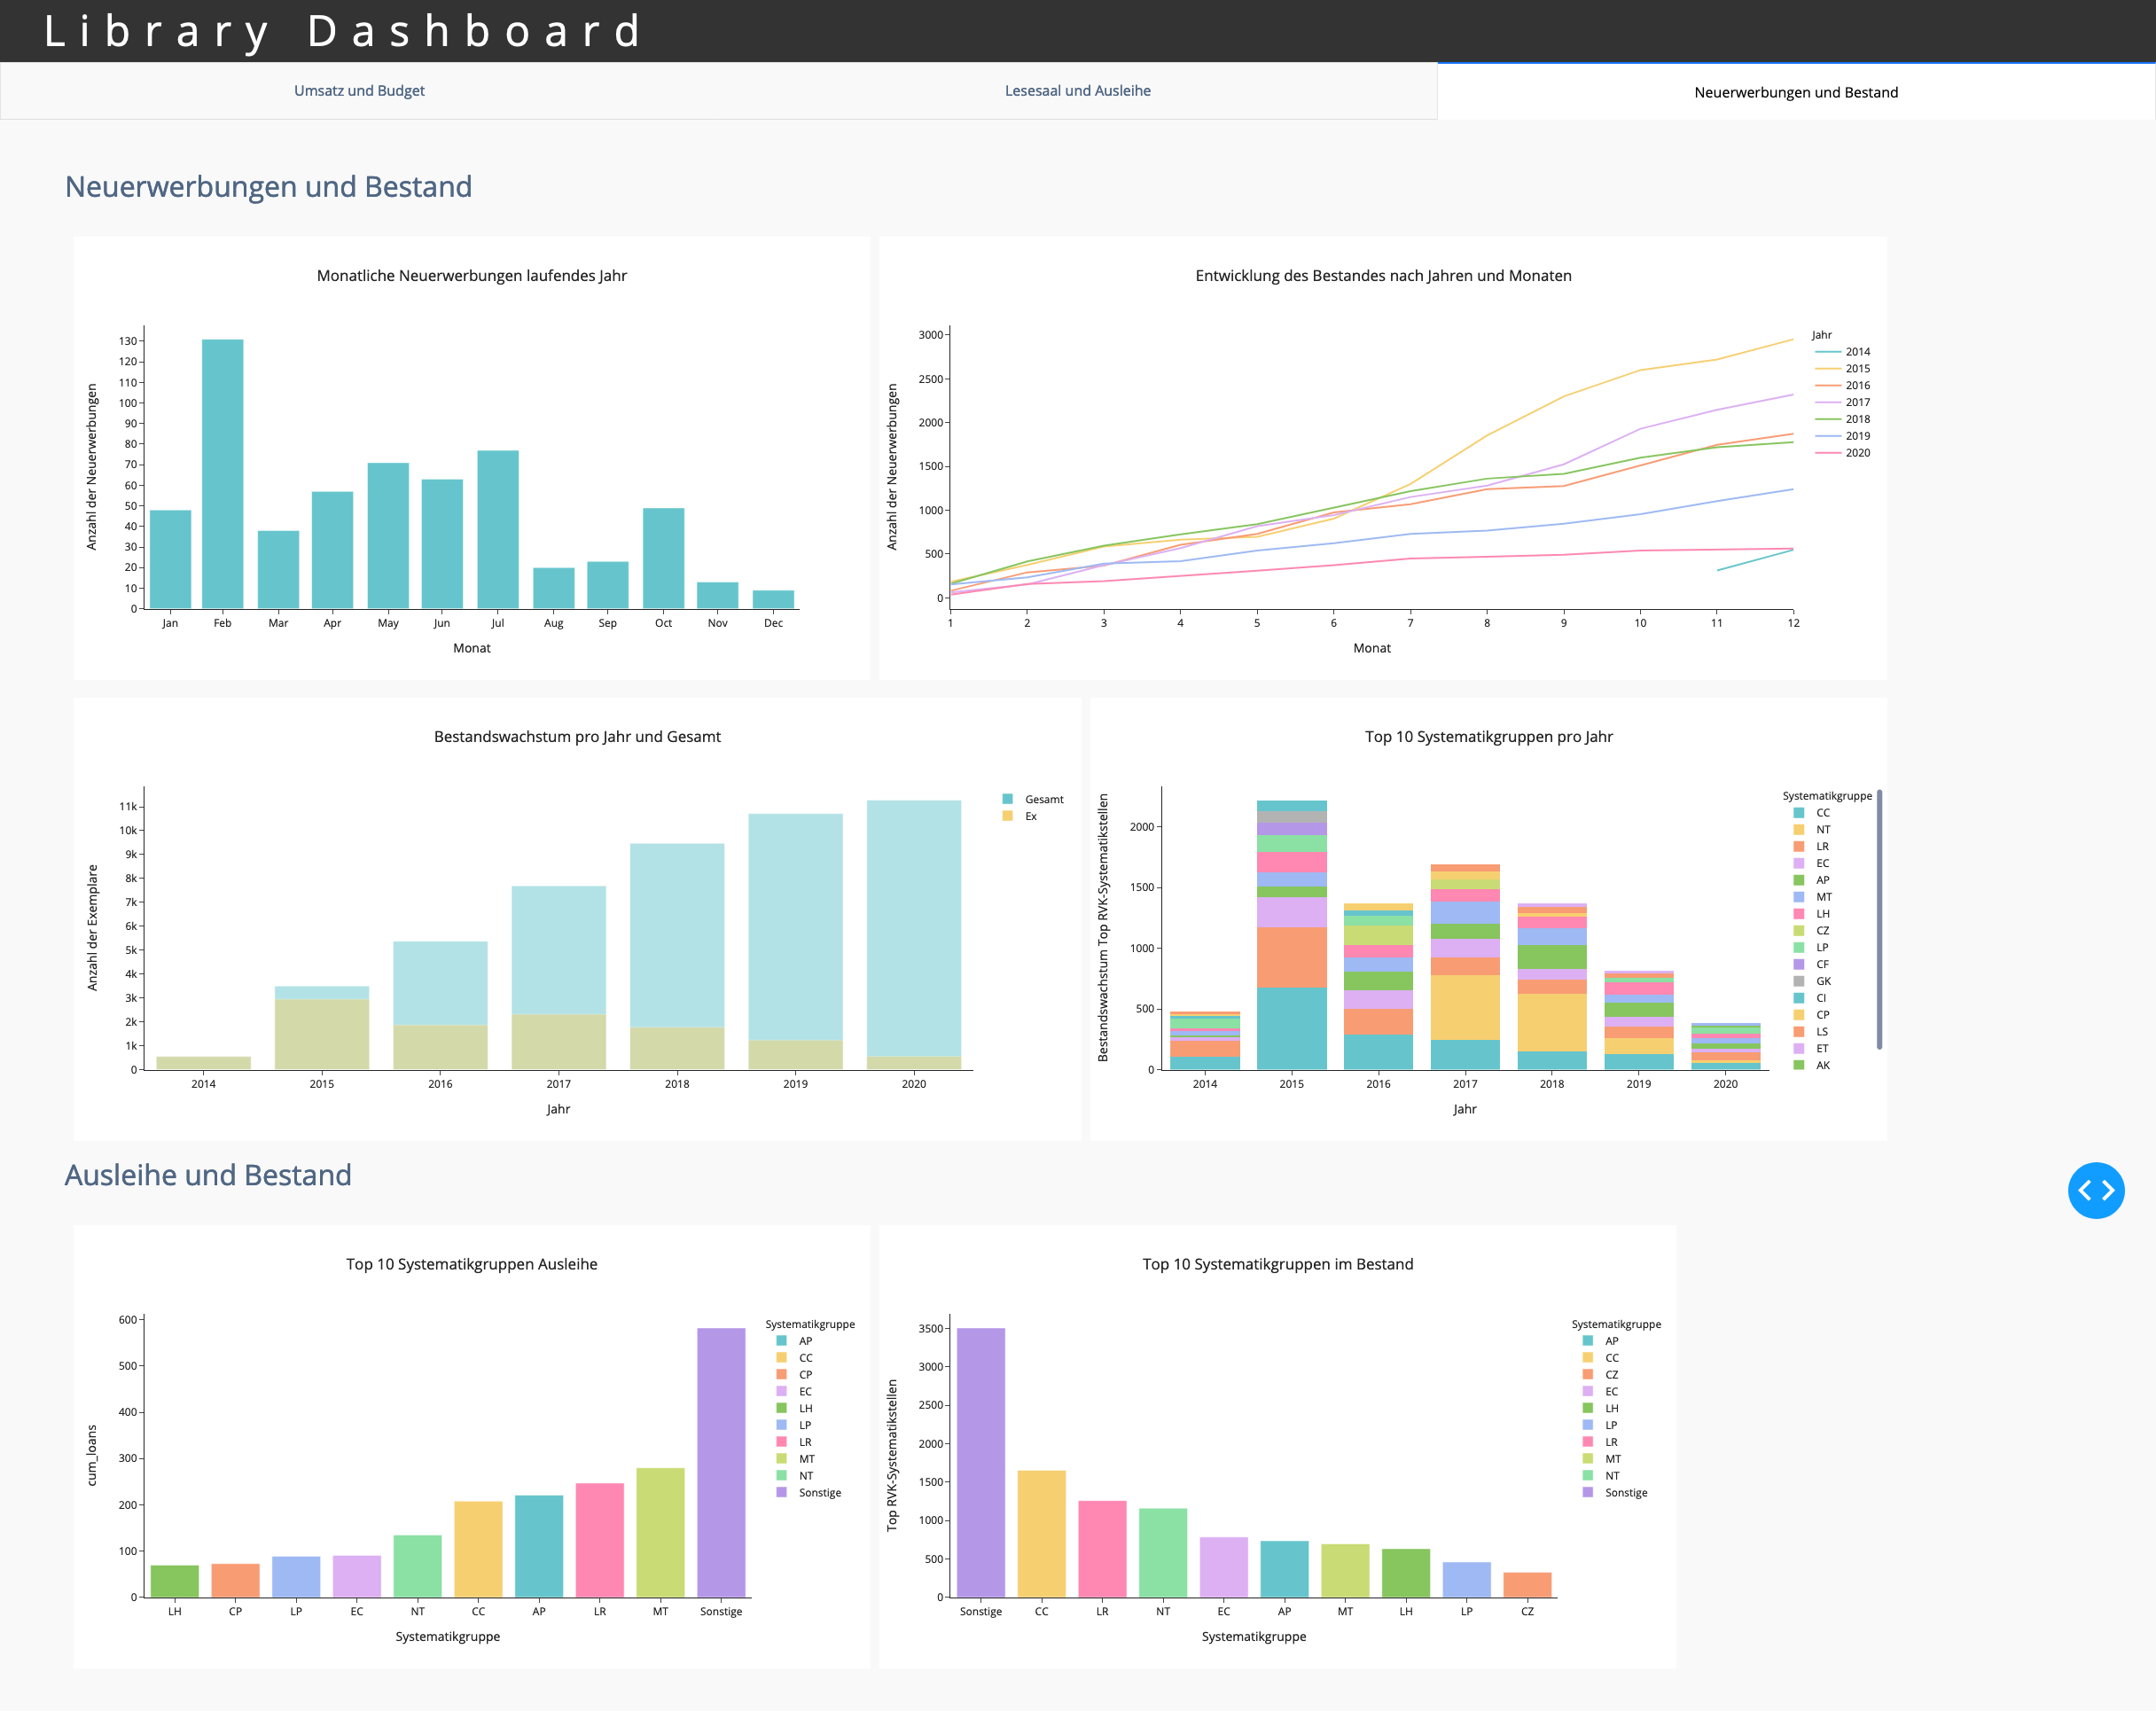
\includegraphics[width=15cm, height=12cm]{tab3}
            \caption{Tab3}
            \label{fig:tab3}
    \end{figure}

    
     



\section{Bewertung}

\subsection{Umgesetzte Anforderungen}
    Folgende Must-Anforderungen wurden erfüllt.
    R1, R2, R3, R4, R5, R7
    F1, F4, F5, F12
    NF5, NF6, 


zur Datenlage 
Ausleihdaten nur auf Zuruf, mtl. Daten bekommen wir erst seit 2021 zu geschickt.
kumulative Daten bei Umsatz/Budget
fehlen der UmsatzDaten für Datenbanken müsste nochmal händisch nachgetragen werden (ca. 20.000 Euro)
Fehlen der Buchservice-Daten (Subito, ...) -> keine Zeit
nur Daten die aus dem CBS/LBS  stammen
fehlen Daten der Online-Zeitschriften

dennoch:
gelungen, die vorhandenen Daten soweit zu importieren, dass mit diesen über das Dataframes Manipulationen und Berechnungen
durchgeführt werden können. Ebenso ist es gelungen eine grafische Oberfläche für die Diagramme anzubieten. Diese Diagramme
sind mit Plotly interaktiv. Es konnte auch ein bisschen interaktivität selber programmiert werden.

Es konnte gezeigt werden, das das gelingt\dots

Den größten Teil der Zeit hat die Datenanalyse gekostet (-> ähnlich Data Science Circle). 
pandas sehr mächtig und aber auch nicht trivial ist. Ziemlich gutes Tool für die Datenanaylyse darstellt.


